% !TEX program = xelatex
% !BIB program = bibtex
\documentclass%
	[type=bachelor,
	 printmode=oneside, % auto
	 bilinguallist = off,
	 seriftoc,
	]{cquthesis}%
\usepackage{cquthesis}

\usepackage{minted}
\setminted[python]{
    linenos=true,
    numberblanklines=true,
    numbersep=5pt,
    gobble=0,
    frame=leftline,
    framesep=2mm,
    funcnamehighlighting=true,
    tabsize=2,
    obeytabs=false,
    mathescape=false
    samepage=false,
    showspaces=false,
    showtabs =false,
    texcl=false,
    baselinestretch=1.2,
    fontsize=\footnotesize,
    breaklines=true,
}
\setminted[matlab]{
    linenos=true,
    numberblanklines=true,
    numbersep=5pt,
    gobble=0,
    frame=leftline,
    framesep=2mm,
    funcnamehighlighting=true,
    tabsize=2,
    obeytabs=false,
    mathescape=false
    samepage=false,
    showspaces=false,
    showtabs =false,
    texcl=false,
    baselinestretch=1.2,
    fontsize=\footnotesize,
    breaklines=true,
}
\setminted[xml]{
    linenos=true,
    numberblanklines=true,
    numbersep=5pt,
    gobble=0,
    frame=leftline,
    framesep=2mm,
    funcnamehighlighting=true,
    tabsize=2,
    obeytabs=false,
    mathescape=false
    samepage=false,
    showspaces=false,
    showtabs =false,
    texcl=false,
    baselinestretch=1.2,
    fontsize=\footnotesize,
    breaklines=true,
}
\usemintedstyle{emacs}

% https://tex.stackexchange.com/questions/60209/how-to-add-an-extra-level-of-sections-with-headings-below-subsubsection
\usepackage{titlesec}
\setcounter{secnumdepth}{4}
\titleformat{\paragraph}
{\normalfont\normalsize\bfseries}{\theparagraph}{1em}{}
\titlespacing*{\paragraph}
{0pt}{3.25ex plus 1ex minus .2ex}{1.5ex plus .2ex}

\usepackage{amsmath}

\graphicspath{{images/}}

\begin{document}

\input{contents/cover}
\makecover %%% 封面部分


\frontmatter %%%前置部分(封面后绪论前)
%% 摘要
\makeabstract
%% 目录,注意需要多次编译才能更新
\tableofcontents
%% 插图索引,可选,如不用可注释掉
% \listoffigures
% \listoffiguresEN
% %% 表格索引,可选
% \listoftables
% \listoftablesEN
% %% 公式索引,可选
\listofequations
% \listofequationsEN
% %% 符号对照表,可选
% \input{contents/denotation}


\mainmatter %%% 主体部分(绪论开始,结论为止)
%* 子文件的多少和内容由你决定(最好以章为单位),基本原则是提速预览、脉络清晰、管理容易。



\chapter{绪论}

\section{机器学习的数学工具}
近年大火的机器学习和人工智能技术,均基于计算机的高计算性能实现,其内容主要包含对数据的处理、分类和预测,以及其对应的算法实现。

具体来说,机器学习\textbf{算法实现}的理论基础多为线性代数和概率论、统计论的相关知识,如回归分析、决策树、极值分析和最值分析、集成和聚类学习等。这些算法再经由计算机的软硬件算法,对处理过程加以优化,最终形成可调用的库供用户使用。例如,计算机的图形计算单元(GPU),其单指令多线程(以万为单位)的特性,决定了其适用于多维数据的快速计,并部署上述的各类算法。经优化,现在的GPU算力通常以GFLOPS(Giga-FLOPS, floating-point operations per second, 每秒10亿次的浮点运算数),实现了相较于CPU更快的发展,同时也促进了机器学习的革新进展。

所谓的\textbf{模型}一般用于解决特定性的问题,如YOLO用于机器视觉的多目标识别及分类,及BERT用于自然语言的语句识别及分类。当然,部分算法的代码实现,由于结合了多种算法思想,故也会被称作基本模型,例如概率图模型。前述模型则整合了多种基本模型,以应对复杂的现实问题。因此,非通用类的人工智能均由机器学习实现,本质仍是对数据的处理。\cite{周志华_2016, Sulmont_2019}

与之相对应,通用类的人工智能有机器学习(即数据处理)和生物神经模拟两类研究方向,但目前仍无突出优势和应用。

\section{人脸识别的社会应用}

人脸识别领域是机器学习视觉处理的重要组成部分,也是应用最广泛、社会争议最大的。虽然其名字中只有“识别”两个字,但其内容却包含了识别、分类甚至于特征替换等。经典的特征替换应用实例是DeepFake,这样一个模型可以将视频内的人脸进行替换,并在相当程度上让人类信以为真。虽然机器学习又可以通过该模型的训练规律,反向判断应用该模型“换脸”的视频,但只需稍微应用对抗学习的方法,机器便能自身演化形成独特的替换算法,而不被检测出规律性。\cite{Guera_2018}像这种引起社会恐慌的例子还有很多,在此就不一一列举。

不可否认的是,各类人脸识别系统在近几年如雨后春笋发展起来,但在真实场景的使用中,受限于硬件、成本等条件,这些系统使用的多半是传统的整体分类算法,其发展更多依靠的是数字处理能力的上升,以及智能终端的广泛普及,并已带来相当多的法理伦理问题。本次实验中,程序对数据集进行特征值提取处理后,再应用分类算法进行人脸识别的算法,也是一种简单的整体分类算法。以openCV库中人脸识别的类 \verb|FaceRecognizer| 为例,其包含Eigenface、Fisherface整体(代数特征)算法,以及LBPH局部特征提取算法。这些算法的不足和优化方向均是与脸部特征无关的图像特征,如人脸朝向、光照方向等。

商用级的人脸识别和应用还是以整体(Holistic)识别算法为主,并使用主成分分析(PCA)、独立成分分析(ICA)、线性判别分析(LDA)等作为识别不相关量,并进行降维的算法。在前沿研究和大数据处理方向,基于神经网络的人脸识别则经过卷积神经网络(CNN)等网络模型,被训练为提取偏好特征的特性(Feature)识别算法。基于神经网络的方案又被称为深度学习,它比传统机器学习需要更丰富多元的数据量,同时需要更多的计算性能,因此也更受人们的关注和争议。\cite{Zhao_2003, Anand_2017}

本次实验中要求以可交互界面(可视化用户界面,GUI)实现的特征脸(Eigenface)分类算法,使用的核心算法是主成分分析。实验成果参考了对应的算法,根据\autoref{cha:fr}详述的系统框架实现了相应的目标。具体的算法原理及性能、参数比较,将在\autoref{cha:bg}讨论。此外,为了对图像处理有基础的了解,本次实验还要求对图片进行色彩空间和空域滤波的预处理,具体结果将在\autoref{cha:re}讨论。









% \chapter{实验结果及分析、讨论}
\label{cha:re}

本章展示的实验数据,可通过调用程序相应部分复现。实验分析部分基于文献搜索结果。

\section{模块单元结果}

\subsection{图像的滤波处理}

对某相机拍摄的PNG图片,读取RGB颜色空间后,处理效果如\autoref{fig:hw1}:(其中从左上角,以先从左到右,再从上到下的顺序标数,第一张图像为原图,第二张图像为最大值取样,第三张图像为平均值取样,第四张图像为加权平均值取样(Luminance))

\begin{figure}[H]
    \centering
    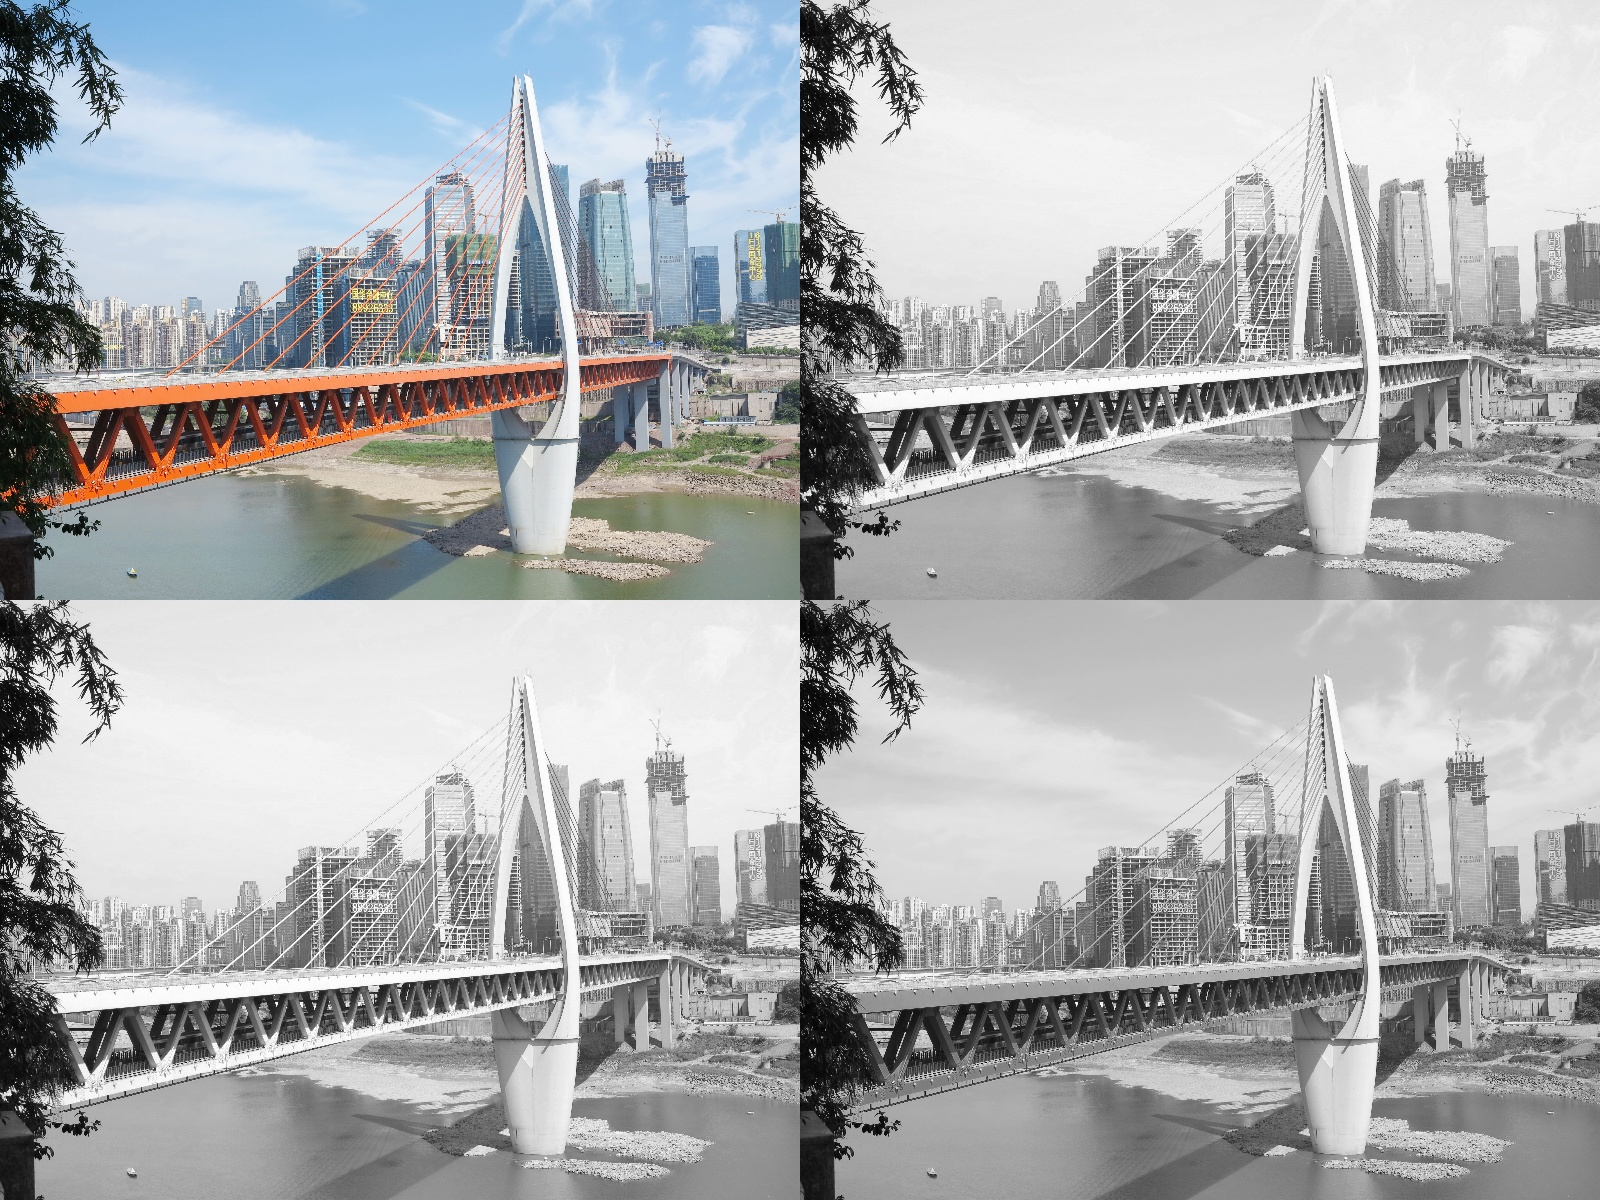
\includegraphics[width=.5\columnwidth]{hw1.jpg}
    \caption{灰度处理实验结果}
    \label{fig:hw1}
\end{figure}

根据人眼观察,在这种情况进行灰度空间转换时,使用加权平均值取样对这张图片的还原度最大,其明度较高的细节,如蓝天白云、红色桥梁等得到了充分保留。而后对数据库内人脸进行同等处理,也得到类似的直观结论。(所以电子行业用这个标准,还是有原因的!)

另外,在使用MATLAB或Python numpy库直接对读取图像进行处理时,很容易忽略数据类型的问题。对于正常的8位3通道图片,各像素点的数据均以\verb|uint8|的形式储存,在加权求和时,由于人脸数据库中图片明度普遍较高,故通道先求和,所得值将超过$2^8-1=255$,导致结果图像数据失真。可以调用平均值函数,或者数据类型转换来无损的解决这个问题。

需要注意的是,若要对这一结果进行深入研究,除了分析观察值外,还要结合其应用场景进行分析。此处,鉴于主流的图像处理工具(Matlab, OpenCV)均使用了Luminance加权平均值取样,故不再具体探讨其对实验结果的影响。为直击重点,本实验也不再探讨直方图优化、伽玛校正的原理,及其与灰度转换相结合的具体作用效果。

\begin{figure}[H]
    \centering
    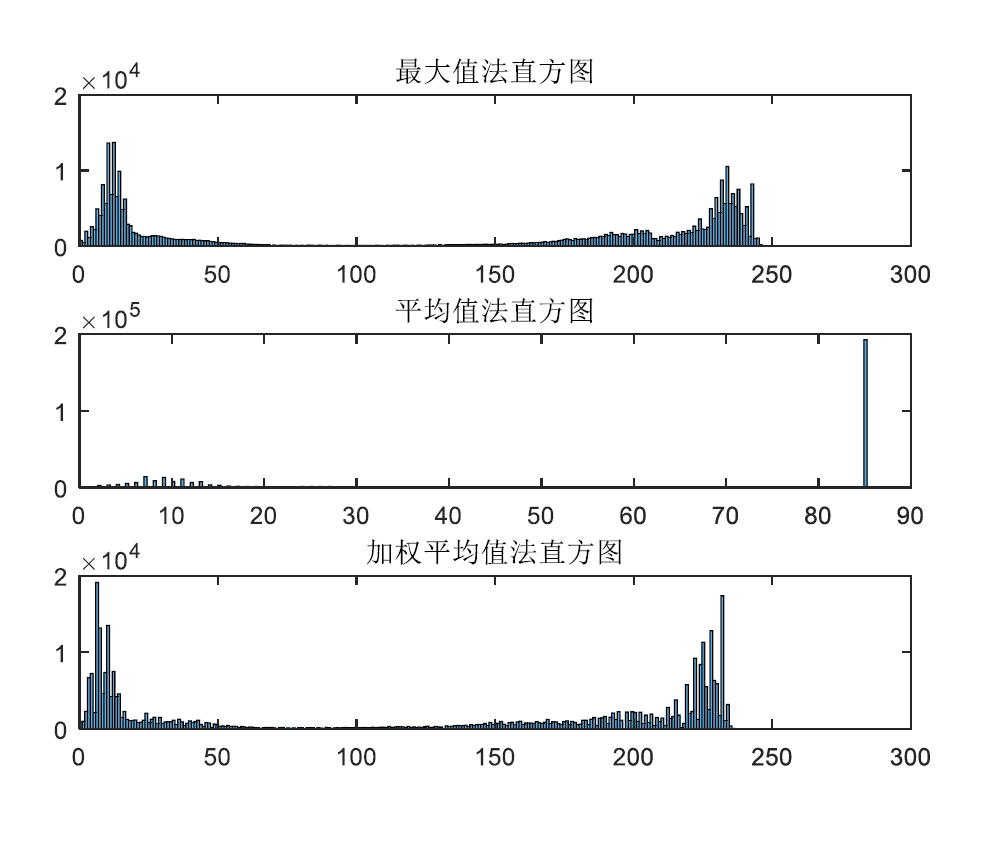
\includegraphics[width=.5\columnwidth]{hw1_add.png}
    \caption{某人脸图片经不同灰度处理后的直方图结果}
    \label{fig:hw1_add}
\end{figure}

\textbf{综上,经分析,程序主模块最终采用本部分的加权平均值取样部分(浮点输出)。}

\subsection{图像的主成分分析}

对数据库中训练库、测试库中的部分照片进行多种去噪处理,并将其图片输出,过中心的平行、垂直线上像素的R通道值的绘图数据,各像素点R通道8位值数据的直方图制作成图表,结果如下。

\begin{figure}[H]
    \centering
    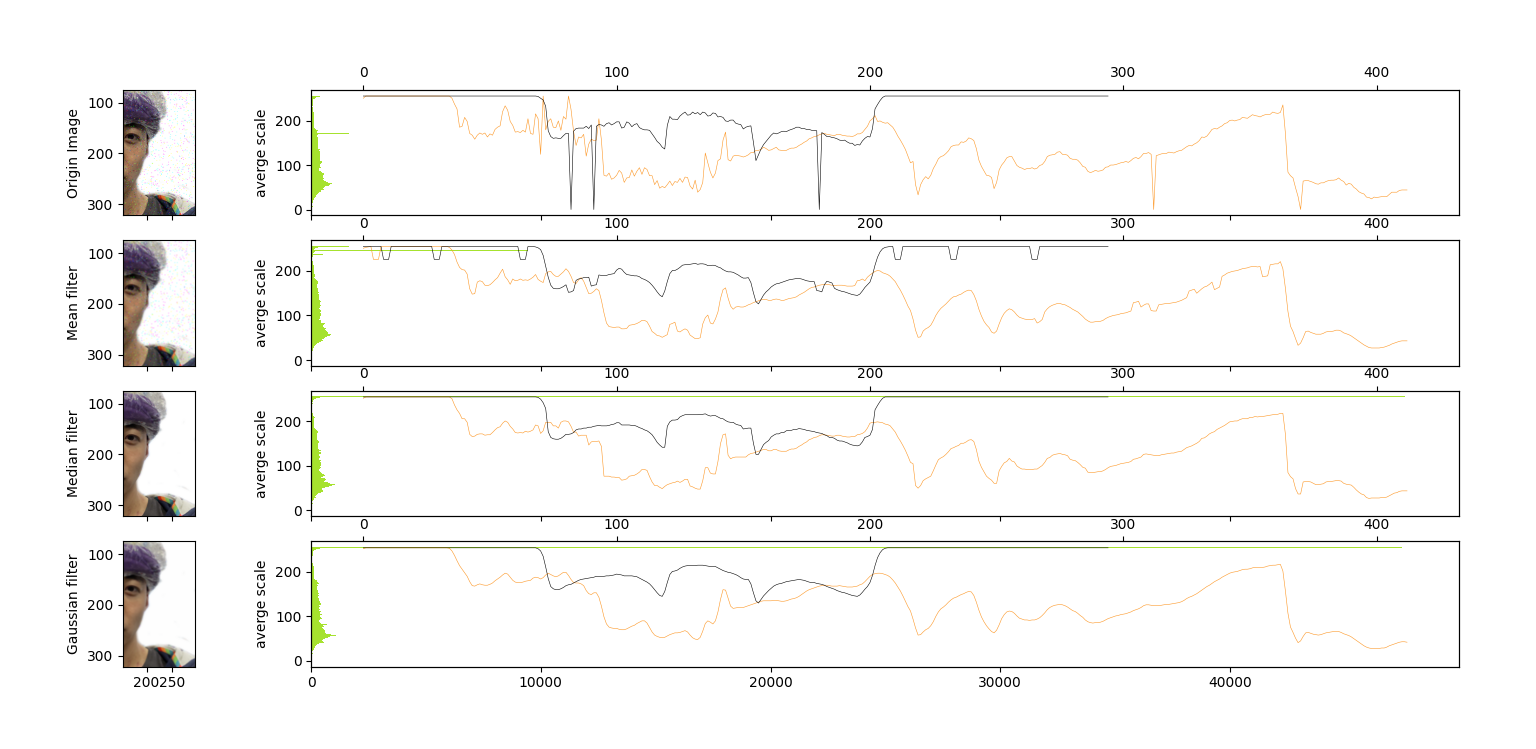
\includegraphics[width=.81\columnwidth]{hw2_fig1.png}
    \caption{三种滤波处理后的输出结果}
    \label{fig:hw2_1}
\end{figure}

\begin{figure}[H]
    \centering
    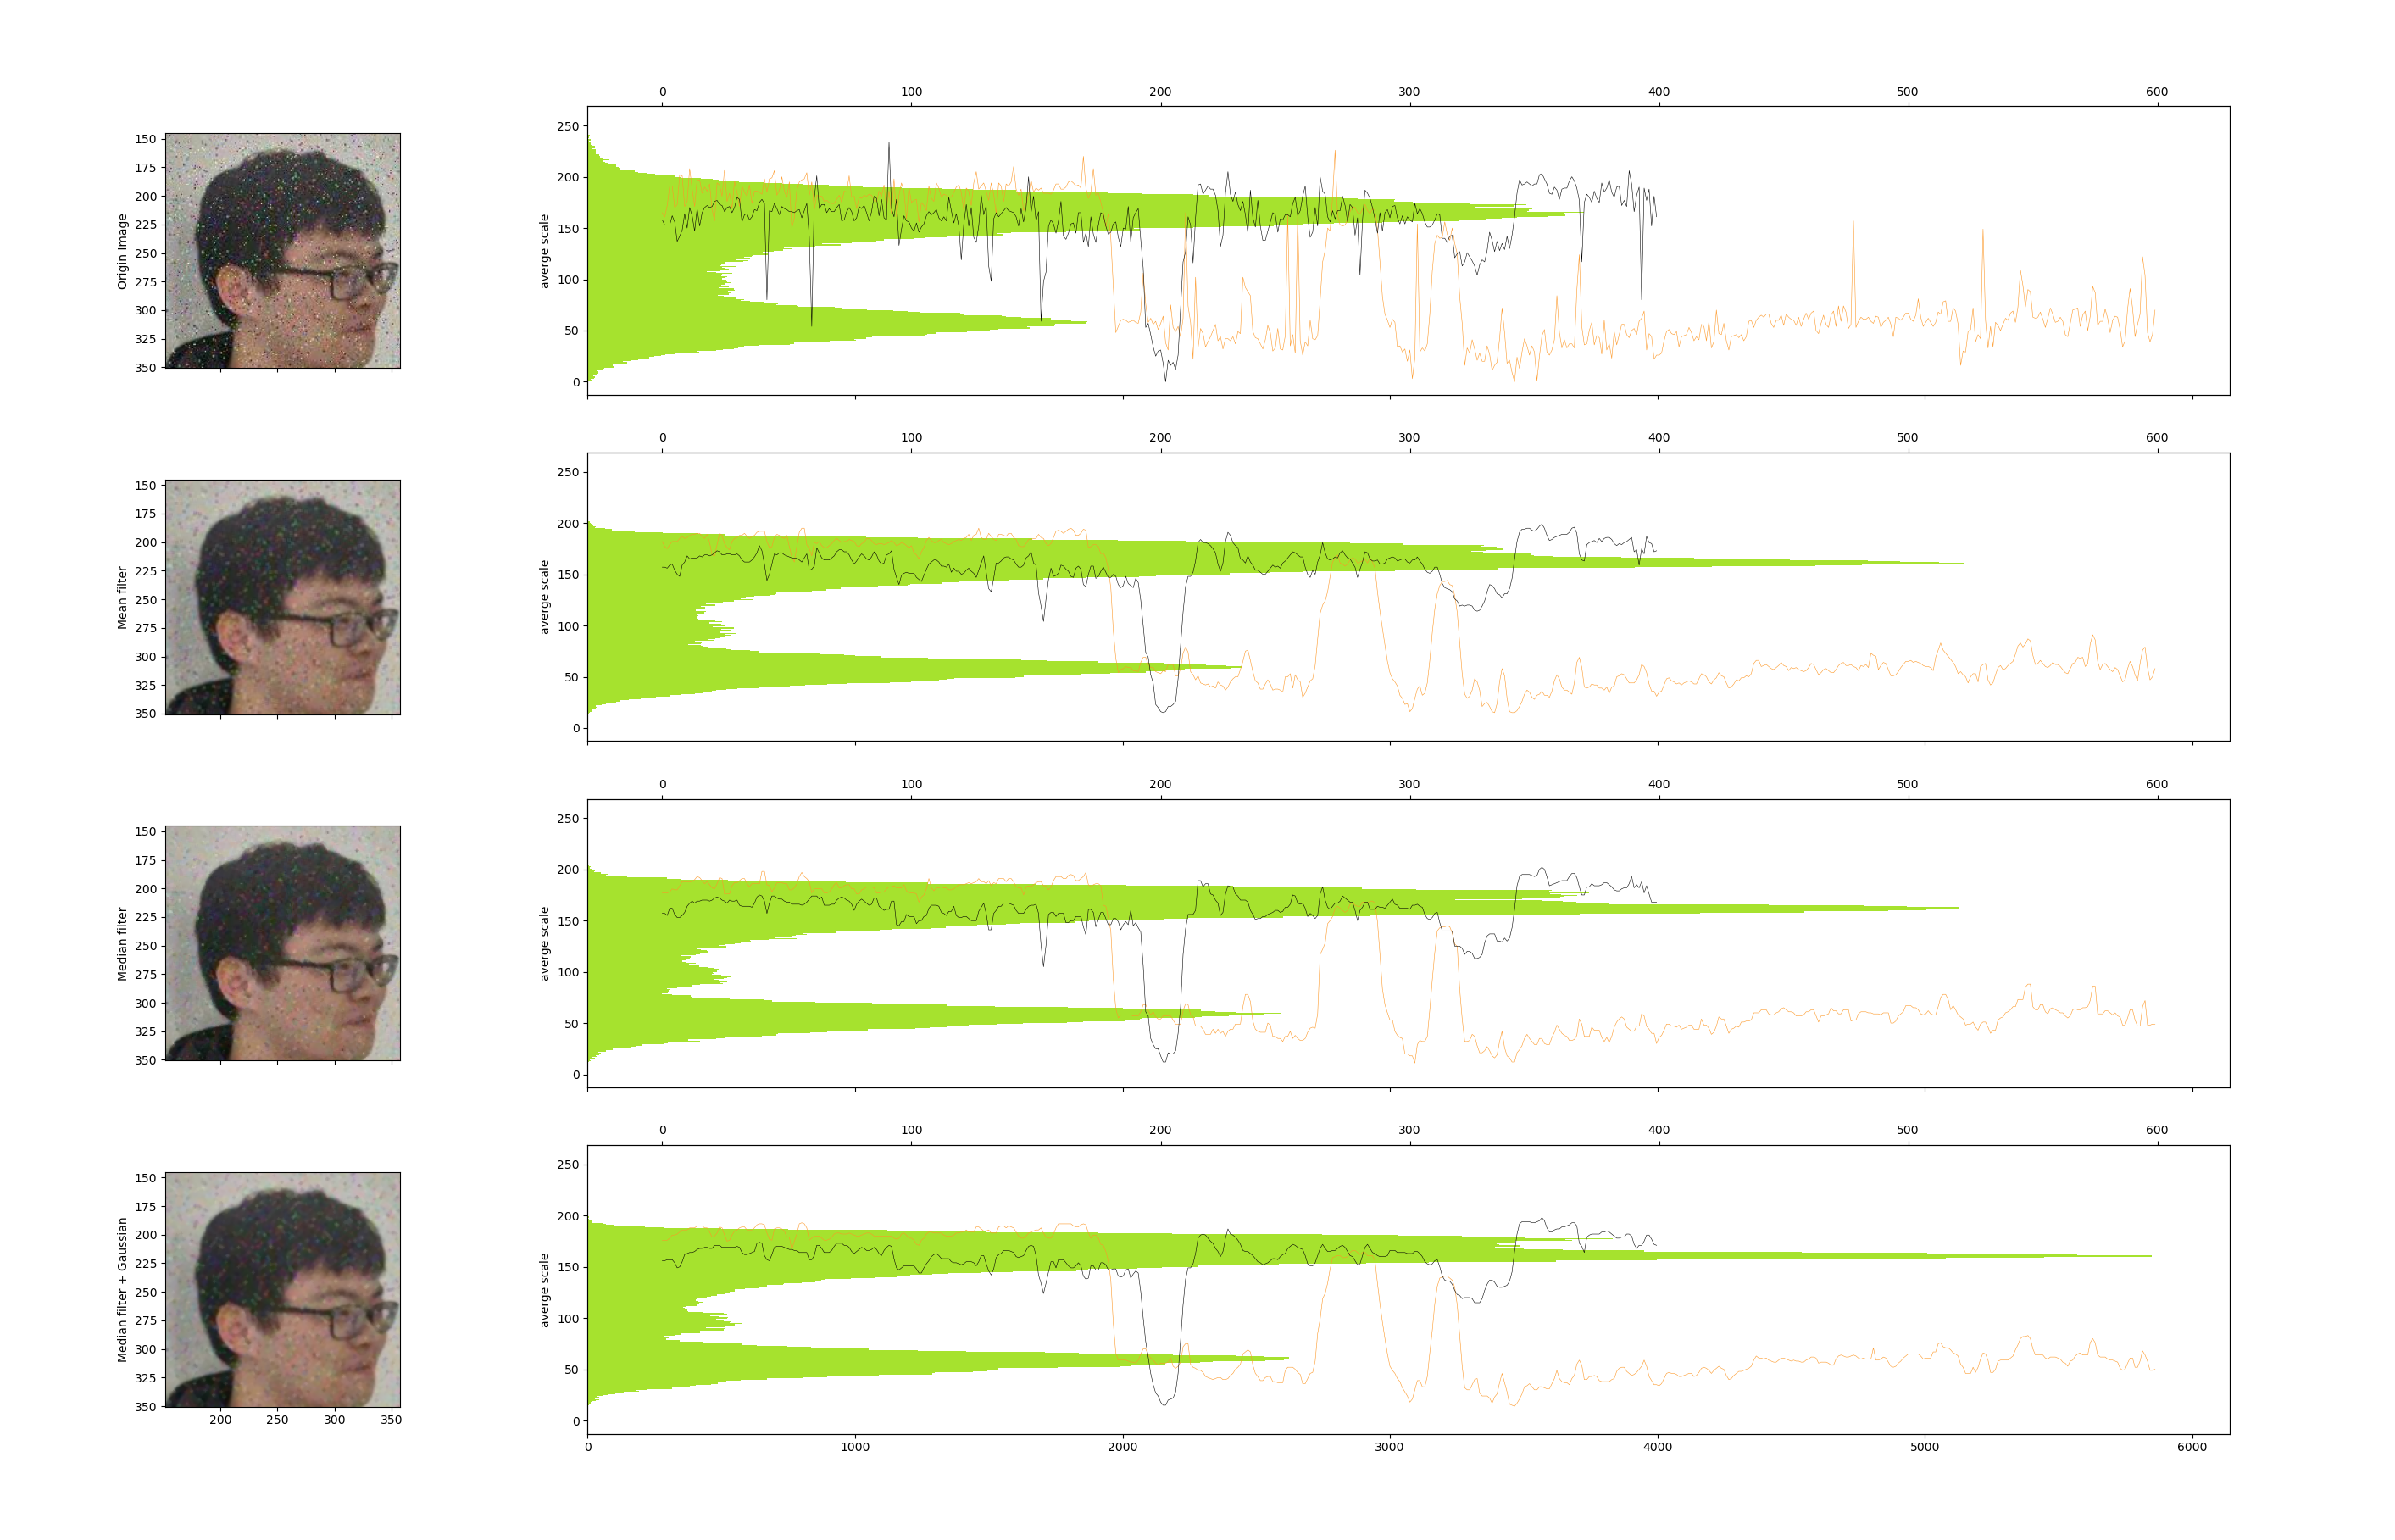
\includegraphics[width=.81\columnwidth]{hw2_fig2.png}
    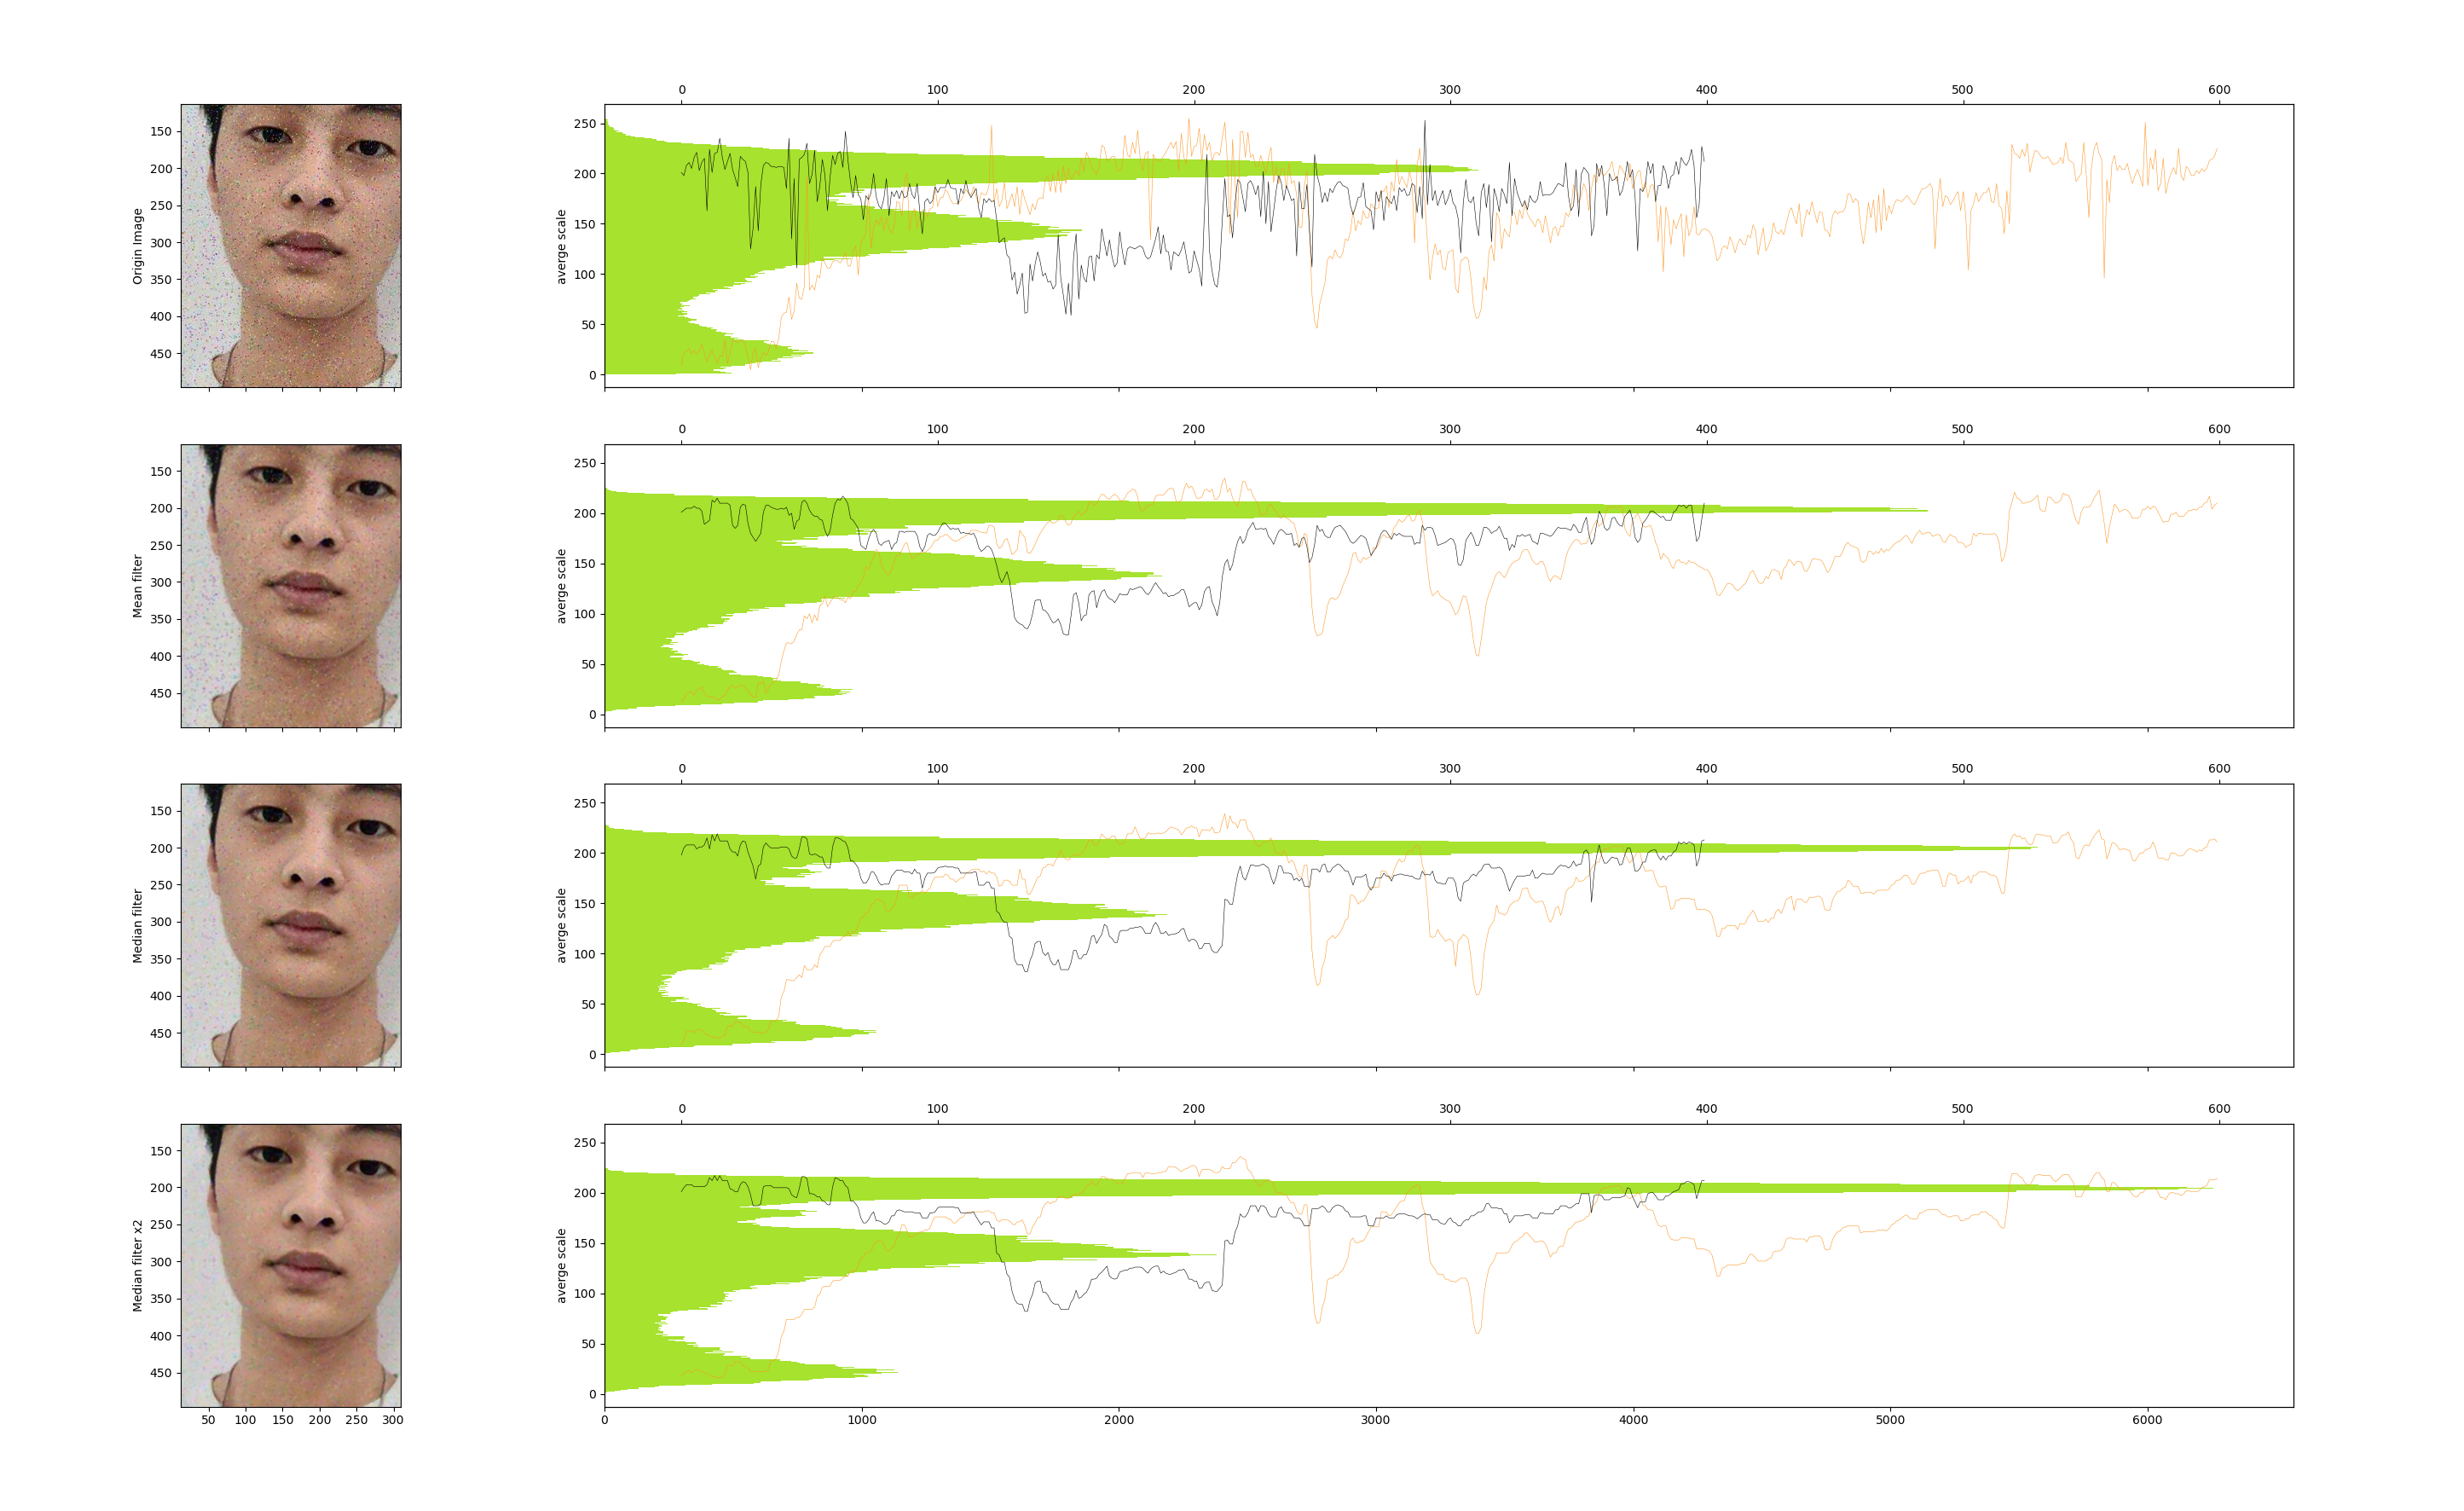
\includegraphics[width=.81\columnwidth]{hw2_fig3.png}
    \caption{分别展示了高斯滤波后中值滤波,两次中值滤波的输出结果}
    \label{fig:hw2_2}
\end{figure}

\autoref{fig:hw2_1}自上而下,展示了原图、均值滤波、中值滤波、高斯滤波的相应结果。可以发现均值滤波对椒盐噪声去除效果不好,另外两种滤波对简单的椒盐噪声去除效果较好。

\autoref{fig:hw2_2}的第一张后两行展示的分别是中值滤波、高斯滤波后中值滤波的输出结果,可以发现高斯滤波反而会增强高密度的椒盐噪声。其第二张后两行展示的分别是一次中值滤波、两次中值滤波的输出结果,可以发现二次中值滤波对噪声还有一定的削减作用。次数再次升高后,效果不再明显。

\textbf{综上,经分析,程序主模块最终采用本部分的中值滤波,并连续调用两次。}

\section{识别、交互系统结果}

\subsection{处理时间}
\label{sec:pca0}

\textbf{在本机}统计了训练模块中较为耗时的两部分:中值滤波处理和样本库主成分分析。不采用中值滤波的耗时为3.4\~4.9s,采用未加速的中值滤波耗时约为18min51s(每张图耗时约5s),numba加速的中值滤波耗时为15.5\~20.4s;主成分分析的耗时为4.2\~9.1s。

识别模块中耗时的主要部分为测试集批量读入,可同等看待。

\begin{figure}[h]
    \centering
    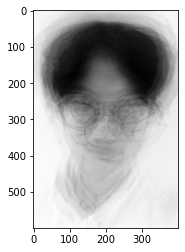
\includegraphics[width=.4\columnwidth]{eig_single.png}
    \caption{单组样本训练得到的第一个主特征,经可视化处理。}
    \label{fig:eig_single}
\end{figure}

\subsection{识别准确度}

对kNN分类算法和选取的主成分进行调整,发现当 $k=4$ 时,主成分最少仅需容纳前$12$维即可达到最佳识别正确率。仅\autoref{fig:class1}所示的样本无法被正确识别。增大主成分维数,识别结果基本不受影响。而增大 $k$ 值会导致部分测试样本匹配到其他类型的人脸。

样本12在$k$、$d$较高时才能被正常识别,如$k=27, d=185$。故样本12的训练集有过拟合的倾向。

\begin{figure}[H]
    \centering
    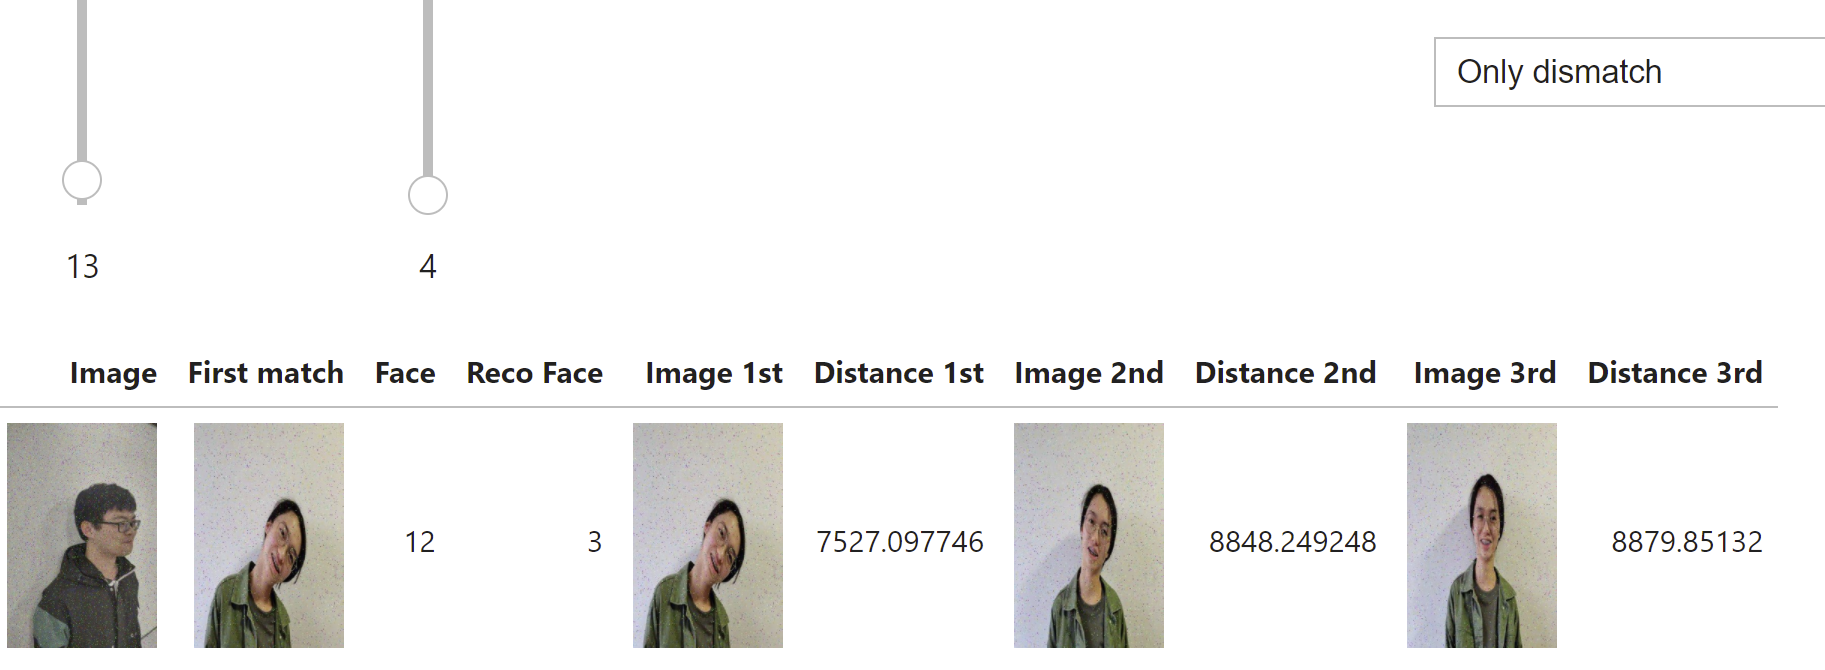
\includegraphics[width=.8\columnwidth]{class1.png}
    \caption{无法匹配的样本图片和识别输出结果}
    \label{fig:class1}
\end{figure}

\section{识别的调整及优化}

下列的数据展示了选取前$d$维主成分和$k$个临近数据集点后的分类情况。注意到有部分测试数据十分接近于训练数据,经查看文件,其中有部分测试图片与训练图片完全一样,另有一些是噪声不同。

\begin{minted}[breaklines]{xml}
d=20, k=4
test face 3 is too close to dataset(s3_1)?
test face 4 is too close to dataset(s4_3)?
test face 9 is too close to dataset(s9_1)?
12 3 [[9.92052951e+03 1.60000000e+01 3.00000000e+00]
 [9.92129420e+03 1.90000000e+01 3.00000000e+00]
 [1.06769758e+04 1.88000000e+02 2.40000000e+01]
 [1.06920015e+04 1.80000000e+01 3.00000000e+00]]
test face 22 is too close to dataset(s22_3)?
Error rate is 0.05.

d=120, k=4
test face 3 is too close to dataset(s3_1)?
7 15 [[[1.41684977e+04 5.80000000e+01 7.00000000e+00]
 [1.62357532e+04 1.23000000e+02 1.50000000e+01]
 [1.70395660e+04 1.20000000e+02 1.30000000e+01]
 [1.92705277e+04 1.22000000e+02 1.50000000e+01]]
test face 9 is too close to dataset(s9_1)?
12 3 [[1.61600607e+04 1.80000000e+01 3.00000000e+00]
 [1.71320333e+04 1.88000000e+02 2.40000000e+01]
 [1.71812421e+04 1.00000000e+01 1.00000000e+00]
 [1.78519738e+04 1.60000000e+01 3.00000000e+00]]
 test face 22 is too close to dataset(s22_3)?
Error rate is 0.1.
\end{minted}

那么我们拿完全不滤去噪声的训练集和测试集来跑跑看呢?好家伙,噪声似乎真的被当作一个特征,留存在高维度的主成分里了。只考虑低维度的主成分,噪声对分类的影响反而不大。

\begin{minted}[breaklines]{xml}
d=6, k=5
test face 1 is too close to dataset(s1_7)?
test face 3 is too close to dataset(s3_1)?
test face 9 is too close to dataset(s9_1)?
13 12 [[ 6279.65703444   175.            23.        ] [11301.58253784   102.            12.        ]]
test face 22 is too close to dataset(s22_3)?
23 5 [[ 8416.09473533   171.            23.        ] [10590.35552612   174.            23.        ]]
Error rate is 0.1.

d=100, k=5
6 3 [[1.34565528e+04 4.40000000e+01 6.00000000e+00] [1.50439833e+04 4.50000000e+01 6.00000000e+00]]
7 15 [[9.86112416e+03 5.80000000e+01 7.00000000e+00] [1.64500187e+04 1.22000000e+02 1.50000000e+01]]
8 22 [[10763.33564653   163.            22.        ] [12367.46637443   162.            22.        ]]
test face 9 is too close to dataset(s9_1)?
13 23 [[2.06595640e+04 1.75000000e+02 2.30000000e+01] [2.58334201e+04 1.70000000e+02 2.20000000e+01]]
23 5 [[2.16220804e+04 1.71000000e+02 2.30000000e+01] [2.55125896e+04 3.20000000e+01 5.00000000e+00]]
Error rate is 0.25.
\end{minted}

\subsection{生成特征向量分析}
\label{sec:eig}

将中值滤波前后的主成分分析工具:特征向量进行比较,更可以发现一些有趣的现象。

\begin{figure}[H]
    \centering
    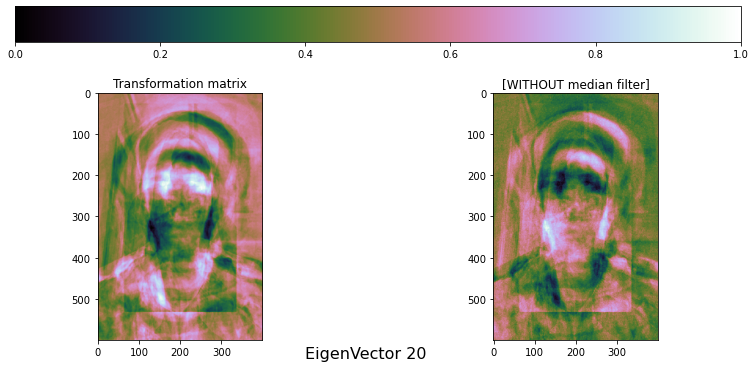
\includegraphics[width=.8\columnwidth]{eig_20.png}
    \caption{$d=20$时的特征向量输出}
    \label{fig:eig_20}
\end{figure}

颜色空间是按照百分比的方式(0~1)对归一化的特征向量进行绘制的。不同方式生成的特征向量,有时候会接近相似,有时会大相径庭,但有时候却会……完全相反?

\begin{figure}[H]
    \centering
    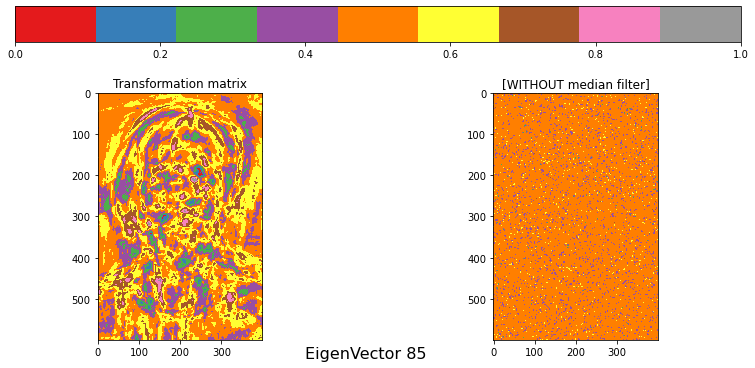
\includegraphics[width=.8\columnwidth]{eig1.png}
    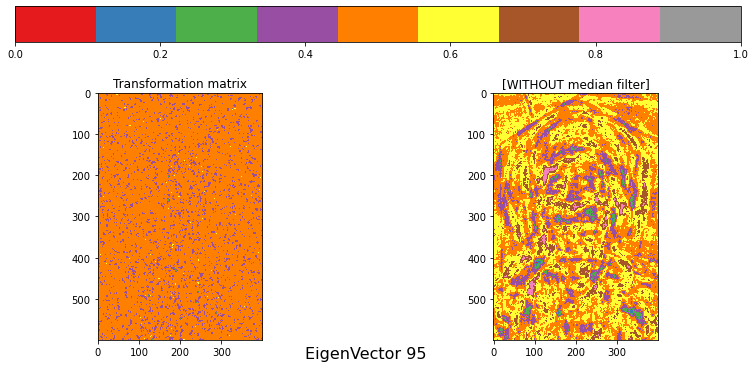
\includegraphics[width=.8\columnwidth]{eig2.png}
    \caption{$d=85$和$d=95$时的特征向量输出}
    \label{fig:eig}
\end{figure}

随着维数增大,两种特征向量里都出现了噪声形成的主成分,且中值滤波前的主成分为噪声的维数更多。这说明生成的噪声过于密集,造成了两个结果:

1.噪声重合形成了一定的规律,并被代数方法所单独识别出来。(这听上去就很无监督学习。)否则,噪声应基本在含有人脸的特征向量中显现。(实际上,两种特征向量里也都有这种情况)

2.套用的中值滤波方式仍不能很好的去除现有的噪声。

那么是时候总结一下了。
% \chapter{反思与总结}

总结本阶段实验,第一项实验给我留下了最深刻的印象。在我之前的认识中,图像的预处理在不同应用领域应当都有最常用的实现方式,甚至于可证明的最优解(State of art)。然后发现这里面的水还是太深了……要考虑的内容比神经网络相关的具体太多,而不是虚无缥缈地调参。同时,我甚至一直以为色彩转灰度只是简单的平均数计算,但对比的图像及其相应的结果都让人大吃一惊。这说明了人眼很容易被图像诓骗,但它又经常对变化敏感。那么,文献收下了,咱慢慢看。

在整理实验报告的时候才注意到滤波器还有很重要的一点没有考虑到,即其作用范围(滤波子的大小)。中值滤波选用稍大的滤波子时,可能会对该数据集的噪声有显著提升的抑制作用。但噪声最好也得用个工具,从信号的角度出发,量化测量一下,不然又得用肉眼看?这可不太好。

在本实验中,数据集有过拟合倾向,因此还应考虑选用其他人脸数据集进行测试,这样或许也能进一步验证我的猜想。不过本次实验也让我迷迷糊糊地认识了协方差矩阵这一个重要概念,老朋友以后见!

感谢老师、助教、同学和开源资料,以及所引参考文献的各作者。该实验的完成缺少不了你们的贡献。


\chapter{实验背景及原理}
\label{cha:bg}
本章将在概论的基础上,基于实验目标,对实验原理进行简单阐述。

\section{实验目标}

\begin{itemize}
    \item 熟悉人脸检测及识别的基本原理和实现方法;
    \item 掌握基于 PCA 方法的人脸识别步骤 、 算法;
    \item 掌握主成分分析 、 特征值 、 特征脸的实现方法 获得对人脸识别的感性认识;
    \item 熟悉数字图像处理常用函数的使用方法及一般数字图像处理系统的设计方法;
    \item 学习 MATLB 软件实现 PCA 算法 进行人脸识别 加深其在其在数字图像处理中解决该类问题的应用流程
\end{itemize}

\section{实验原理概览}

完成本实验,需要了解图像数字化的基本知识。\textbf{从数学的角度出发},数字图片可以看作一个二元函数$f(x, y)$,其中$x, y$是图像的坐标,每组坐标代表着数字图片的一个“像素点”,而函数导出值$f$则是当前像素的强度数据(intensity value),通常来说是一个三元数据。因此,可以认为数字图片完成了二维平面向三维空间的投影。\cite{Tyagi_2018}\textbf{从信号的角度出发},可以将图像数字化看作是采样和量化两个空域处理的过程。采样是连续的二维模拟信号被离散为像素点的过程,量化则是连续的强度数据继续被离散为指定采样位(一般为8位)数据的过程。

本实验的灰度处理,正是对图片的颜色空间即强度数据进行研究。实验的滤波处理,则聚焦于噪声处理方向。实际上滤波还会被用于图像边缘特征、细节特征的增强,模糊处理、特征/频域水印等风格化处理。实验的主成分分析,则要运用到概率论和矩阵论的有关知识。

数字音频和数字图片在数学和信号角度上只有维数的区别,因此对他们的基础研究是相通的。数字处理除了在数学和信号处理中有重要意义外,还在信息提取、压缩、数据传输等各方面有着广泛的应用。

\section{子任务模块}

\subsection{图像的灰度处理}

花花世界无奇不有,但要将不同颜色通道的数据整合到一个通道,\inlinecite{Kanan_2012}指出也是具有挑战性的。下列给出实验中用到的三种由RGB通道取样到灰度通道的方式。(均不考虑伽马处理)

\begin{figure}[H]
    \centering
    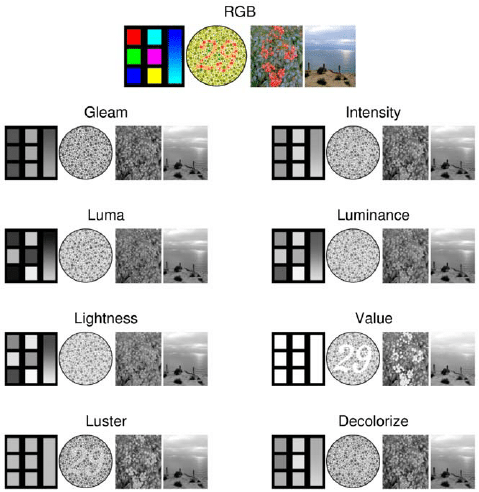
\includegraphics[width=.5\columnwidth]{the0.png}
    \caption{常见灰度处理方法及其应用结果\cite{Kanan_2012}}
    \label{fig:the0}
\end{figure}

\begin{itemize}
    \item 最大值取样(Value in HSV, Hue, Saturation, and Value)
    \begin{equation}
        G = \max \{R, G, B\}
    \end{equation}
    \item 平均值取样(Intensity)
    \begin{equation}
        G = \overline{ \{R, G, B\} }
    \end{equation}
    \item 加权平均值取样(Luminance, Follow CCIR 601)
    \begin{equation}
        G = 0.299 \cdot R + 0.587 \cdot G + 0.114 \cdot B
    \end{equation}\eqlist{Luma均值取样}[Luma均值取样]
\end{itemize}

\subsection{图像的滤波处理}

从频域上来看,滤波可分为低通和高通两种滤波类型。噪声可能是人为赋予,但更一般的情况下是感光元件和数据压缩处理时产生的,并一般在频域的高频段分布。故使用一些低通滤波可以减弱不同类型的噪声干扰。

\begin{figure}[H]
    \centering
    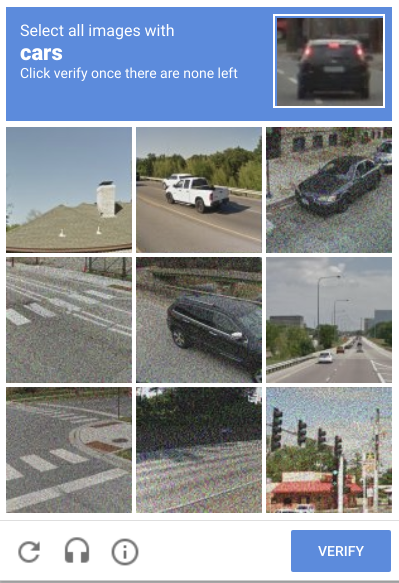
\includegraphics[width=.5\columnwidth]{the1.png}
    \caption{在验证码的识别图像中出现的对抗噪声(Adversarial Noise)\cite{Lambda_2018}}
    \label{fig:the1}
\end{figure}

本实验中用到了三种滤波方法:设$f(i, j)$表示$(i, j)$所代表的像素点的强度数据,$k$表示滤波在二维空域上的应用范围。实验时均使用的是小滤波子(即$k=1$)。

\subsubsection{均值滤波}
\label{sec:mean-filter0}

当$k=1$时,均值滤波可表示为:

\begin{alignat}{3}
    f(i, j) =& \rm{mean} \{& \forall{i_0, j_0} \in \{ x \in {Z} | &  -k \leq x \leq k\}~&~f(i + i_0, j + j_0)\}\\
    =&\rm{mean} \{& f(i - 1, j - 1),& f(i - 1, j),& f(i - 1, j + 1)\notag\\
    && f(i, j - 1),& f(i, j),& f(i, j + 1)\notag\\
    && f(i + 1, j - 1),& f(i + 1, j),& f(i + 1, j + 1)\}\notag
\end{alignat}

均值滤波(mean filter)常用于图像平滑和模糊,对随机噪声的去除性好。

\subsubsection{中值滤波}
\label{sec:median-filter0}

当$k=1$时,中值滤波可表示为:
\begin{alignat}{3}
    f(i, j) =& \rm{med} \{& \forall{i_0, j_0} \in \{ x \in {Z} | &  -k \leq x \leq k\}~&~f(i + i_0, j + j_0)\}\\
    =&\rm{med} \{& f(i - 1, j - 1),& f(i - 1, j),& f(i - 1, j + 1)\notag\\
    && f(i, j - 1),& f(i, j),& f(i, j + 1)\notag\\
    && f(i + 1, j - 1),& f(i + 1, j),& f(i + 1, j + 1)\}\notag
\end{alignat}\eqlist{中值滤波}[中值滤波]

中值滤波(median filter)可有效除去脉冲噪声,如\autoref{sec:dataset}中描述的数据集。\cite{Arakawa_1996}

\subsubsection{高斯滤波}
\label{sec:gaussian-filter0}

高斯滤波核可由下式计算:

\begin{equation}
    f(i,j) =\frac{1}{2\pi\sigma^2}e^{-\frac{i^2+j^2}{2\sigma^2}}
\end{equation}

高斯滤波(mean filter)也常用于图像平滑和模糊,对频域高斯噪声的去除性好。此处的高斯滤波为低通高斯滤波。

\subsection{图像的主成分分析}

\subsubsection{协方差矩阵}

协方差各项为$Cov(\vec x, \vec y)$。此处不考虑协方差矩阵的系数。

可证得协方差矩阵的特征向量按特征值从大到小排序后,各向量归一化(normalization, 2-范数为零)后得到的矩阵即为到主成分空间的变换矩阵。

\subsubsection{变换矩阵的计算}

鉴于数据规模大,我们需要使用矩阵SVD分解的知识来快速、省空间地得到主成分空间的变换矩阵,即原矩阵的协方差矩阵的特征向量矩阵(经排序和归一化处理)。

首先对矩阵中心化(centralization)处理,这使得\autoref{align:import}结果是方差相乘,满足协方差矩阵的定义。(此处数据都是行向量)

\begin{align}
    X_{c(m\times n)} &= X_{m\times n} - \overline{X_{m\times 1}} \cdot [1]_{1\times n} \\
    Cov_{n \times n} &= X^T_c \cdot X_c \label{align:import}
\end{align}

若真要这么计算,n所代表的高维数将让计算机难以下手。但由SVD分解知识可得(此处省略系数):

\begin{align}
\begin{split}
    \rm{eig}(Cov_{n \times n}) &= \\
    \rm{eig}(X^T_c \cdot X_c) &= X_C \cdot \rm{eig}(X_c \cdot X^T_c)
\end{split}
\end{align}\eqlist{SVD导出}[SVD导出]

至此,求出$ T_{m \times m} = X_c \cdot X^T_c $,再进行特征值求解(Listing \ref{listing:dev}),便可以将高维图片向量组乘以变换矩阵,得到各向量降维后的各主成分了。\cite{Abdi_2010, orfanidis_2007, Wold_1987, Pearson_1901}

另外,由于要用到的主成分空间维数不高,还有人提出贪心的算法优化计算。\cite{王晓伟_2013}

\subsubsection{样本分类方法}

k近邻算法(kNN, k Nearest Neighbor)在非监督学习(聚类)中称为k平均算法,其计算样本到各数据点的欧式距离,并选择距离最近的k个数据点,将出现最多的类别作为样本所属分类。该分类算法效果依赖于选择的k值,且因其懒惰学习的特性,导致分类效率低。\textbf{本实验没有采用kNN的任何优化变种,同时出现多个最大值时对k进行缩小迭代},其中欧氏距离:\cite{Guo_2003}

\begin{equation}
    d = \Vert\vec x - \vec y\Vert = \sqrt{\sum^{n}_{i=1} {(x_i - y_i)}^2}
\end{equation}


注意到该方案和近邻成分分析(NCA, Neighbourhood components analysis)原理虽然相似,但缺少状态估计环节和梯度分析。

该方案用于给定数据及标签,对样本进行分类的任务,故此时的kNN分类算法充当着有监督学习的工具。

除了使用kNN分类算法,支持向量机(SVM)也经常用于对数据更主动的分类,且预期效果比人工对$k$调参要好得多。\cite{Cortes_1995, techping_2018, Hu_2019}
%\include{contents/analysis}
\chapter{主模块设计}
\label{cha:fr}
根据实验要求,实验成果应整合算法子任务模块的有关功能,并需要进行完备的主模块设计。本章将介绍整体设计及其设计原因。

\section{系统框架设计}

实验成果的软件系统整体框架图如下:

\begin{figure}[H]
    \centering
    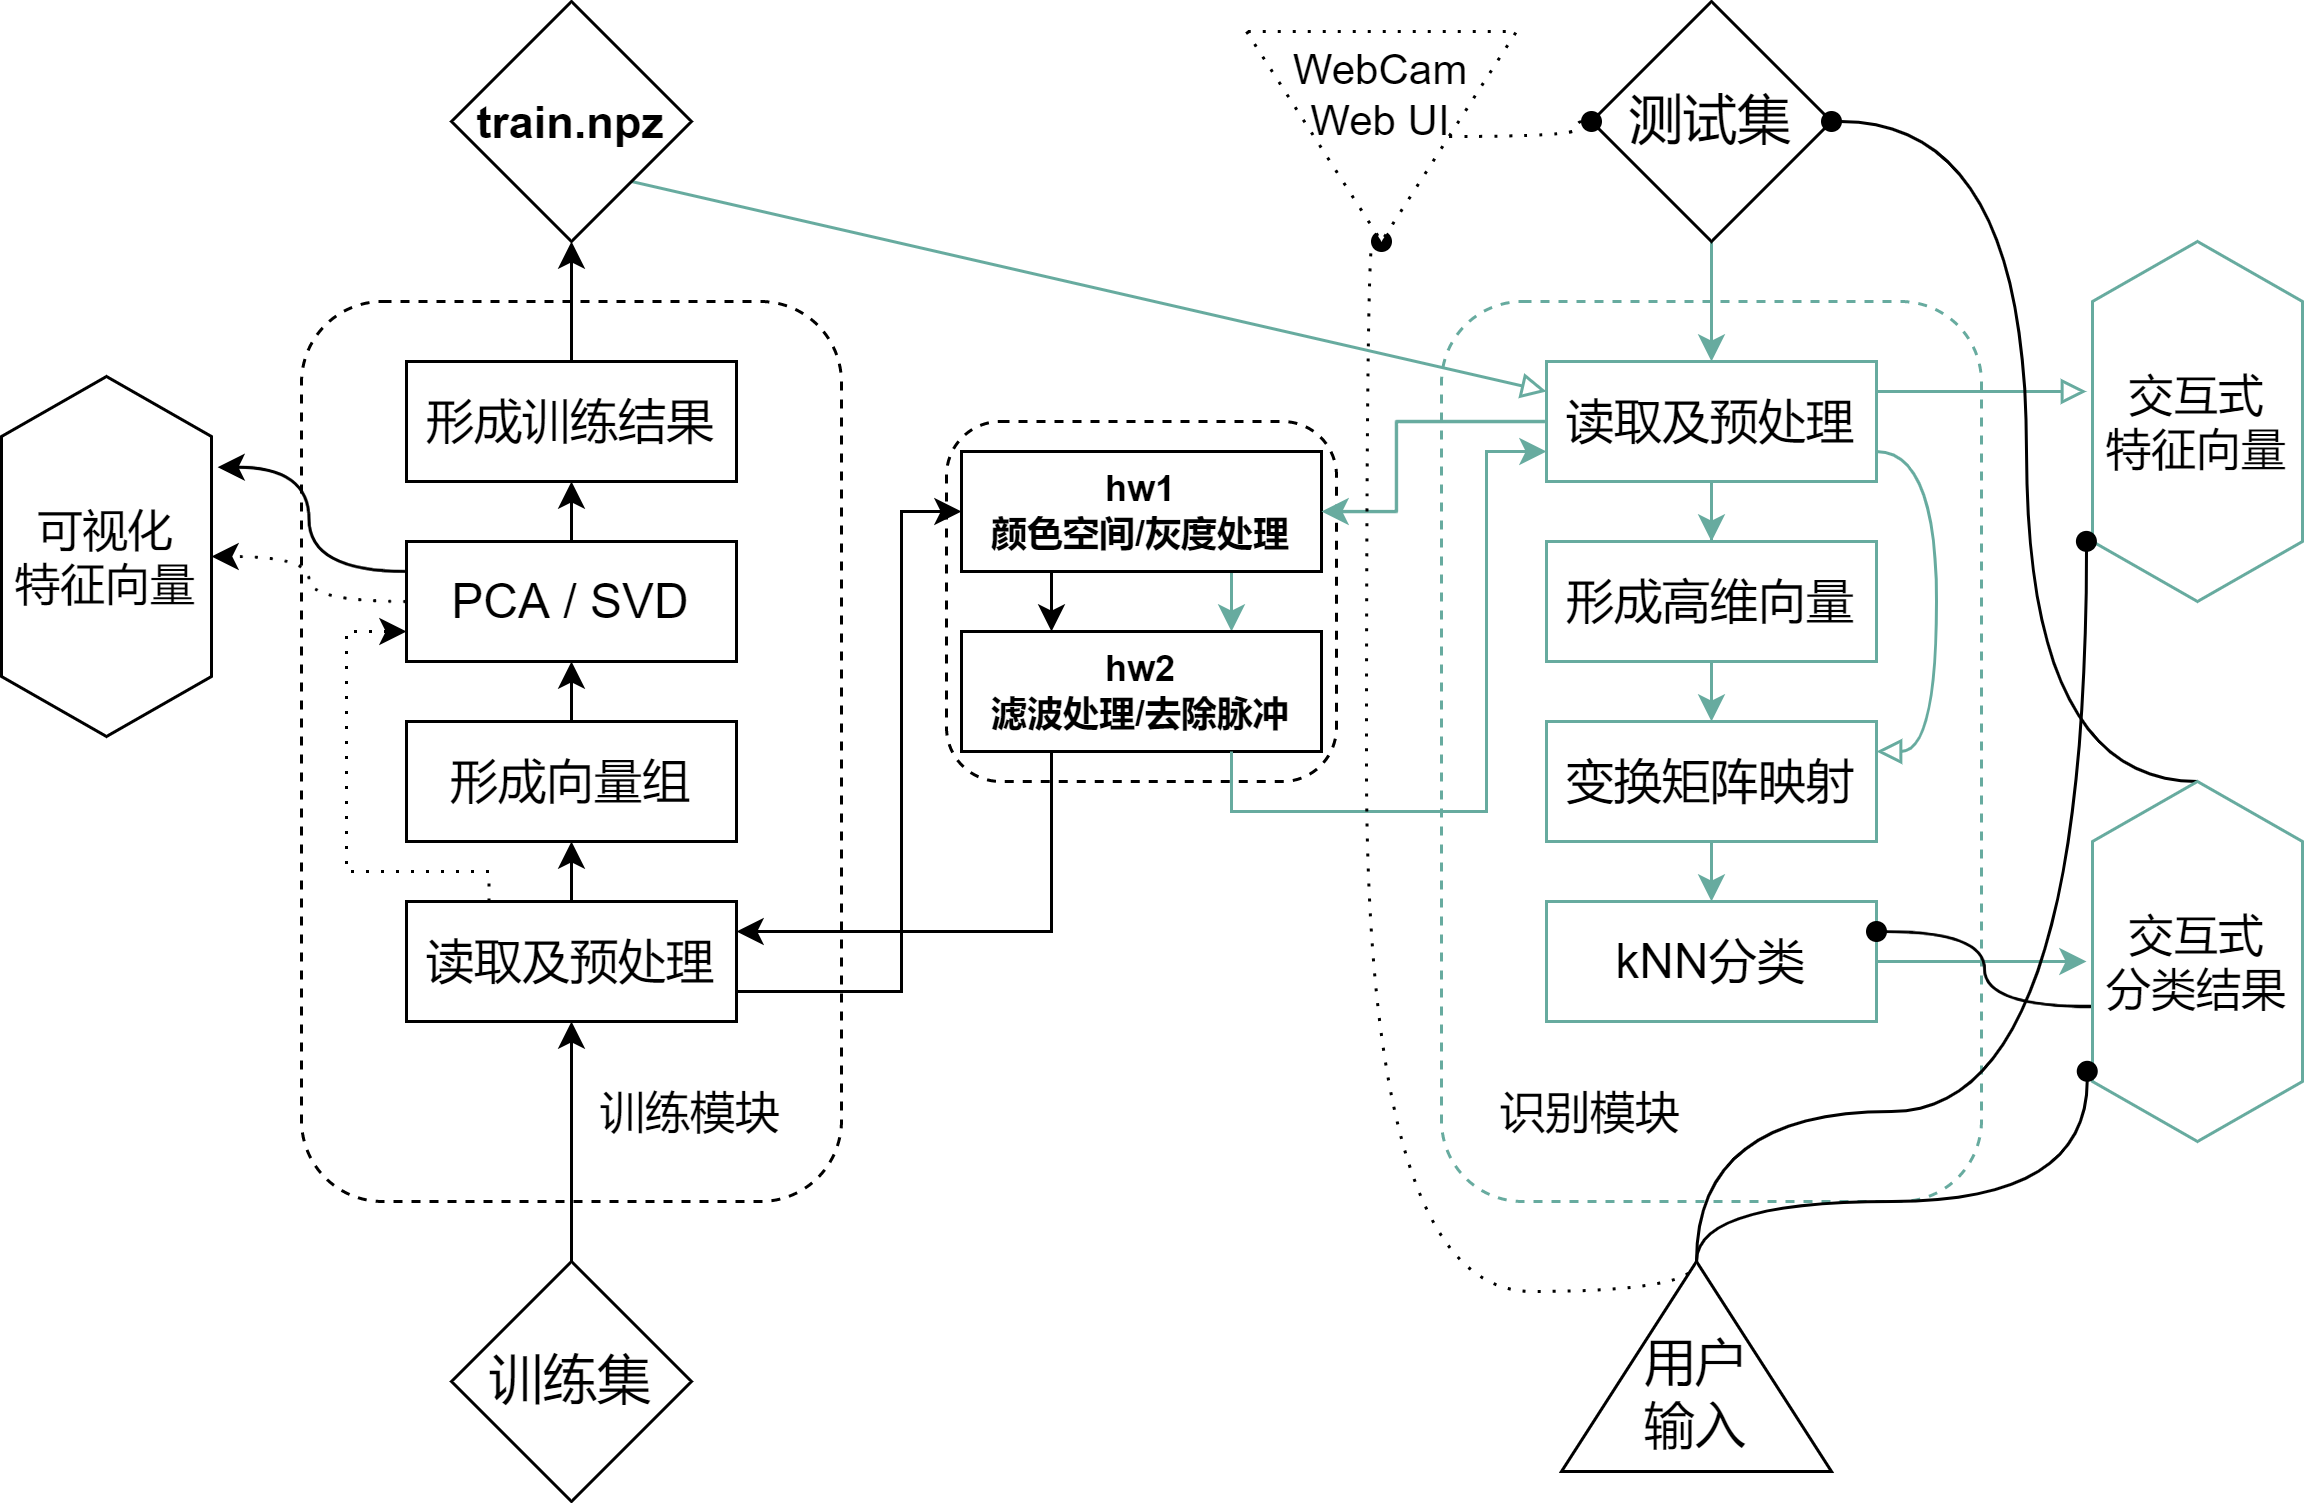
\includegraphics[width=.9\columnwidth]{framework.png}
    \caption{软件框架设计图}
    \label{fig:framework}
\end{figure}

\begin{itemize}
    \item 直接可视化特征向量:对部分单一人脸进行了主成分分析,见\autoref{fig:eig_single}。
    \item WebUI:本软件预留了网页端的相关接口。
\end{itemize}

\subsection{训练集和测试集}
\label{sec:dataset}

数据集均为\verb|600x400|的有露出人脸照片,格式为\verb|.jpg|,有两组样本具有加入噪声后的白边,有一组样本照片部分经过了一次逆时针旋转。约9成的照片加入了随机生成的彩色椒盐噪声。
\begin{itemize}
    \item 在空域中,椒盐噪声分别指极暗或极亮的像素点,且明显不属于原照片的内容,其又名脉冲噪声。
    \item 此处的彩色噪声,指任意单通道的值极大或极小。
\end{itemize}

\begin{figure}[H]
	\begin{minipage}{0.45\textwidth}
		\centering
		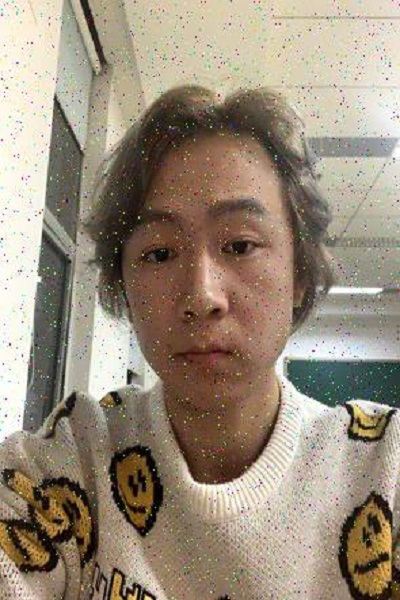
\includegraphics[width=.75\columnwidth]{s26_7.jpg}
		\caption{含椒盐噪声。本组样本的照片,含戴上眼镜与未带眼镜两种。}
	\end{minipage}\hfill
	\begin{minipage}{0.45\textwidth}
		\centering
		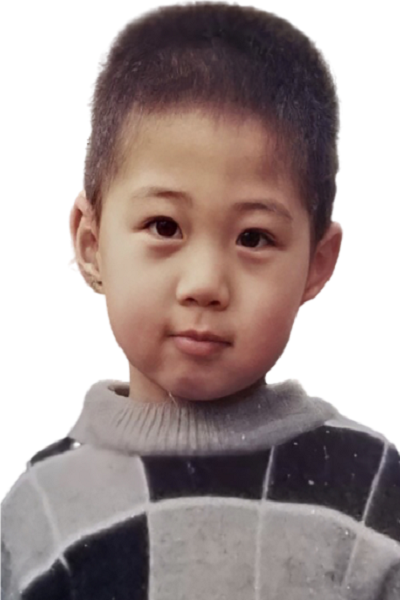
\includegraphics[width=.75\columnwidth]{s13_9.jpg}
		\caption{不含椒盐噪声。本组样本的照片,含不同年龄形态。}
	\end{minipage}
\end{figure}

\section{用户交互框架设计}
\label{sec:ui}

本软件共有两个交互窗口,等待用户输入,见\autoref{fig:ui}。

\begin{figure}[H]
    \centering
    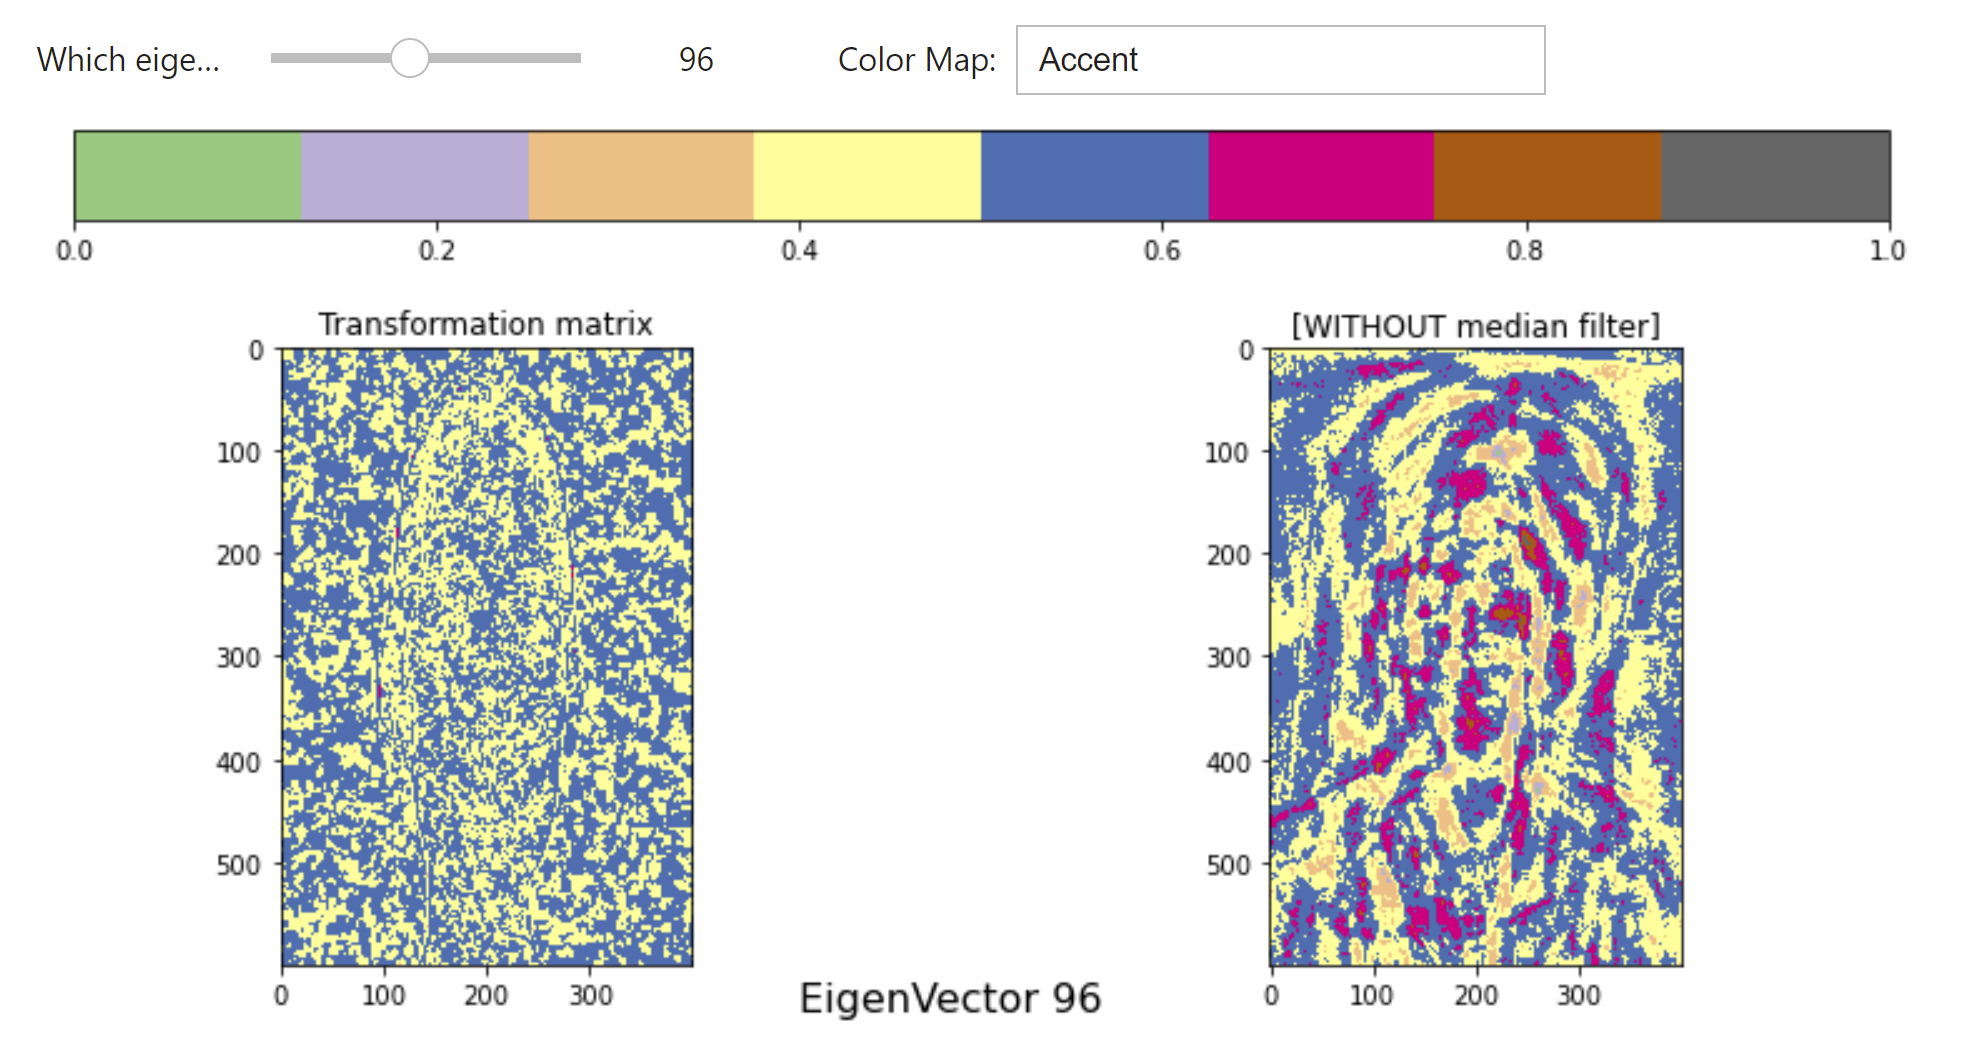
\includegraphics[width=.6\columnwidth]{ui1}
    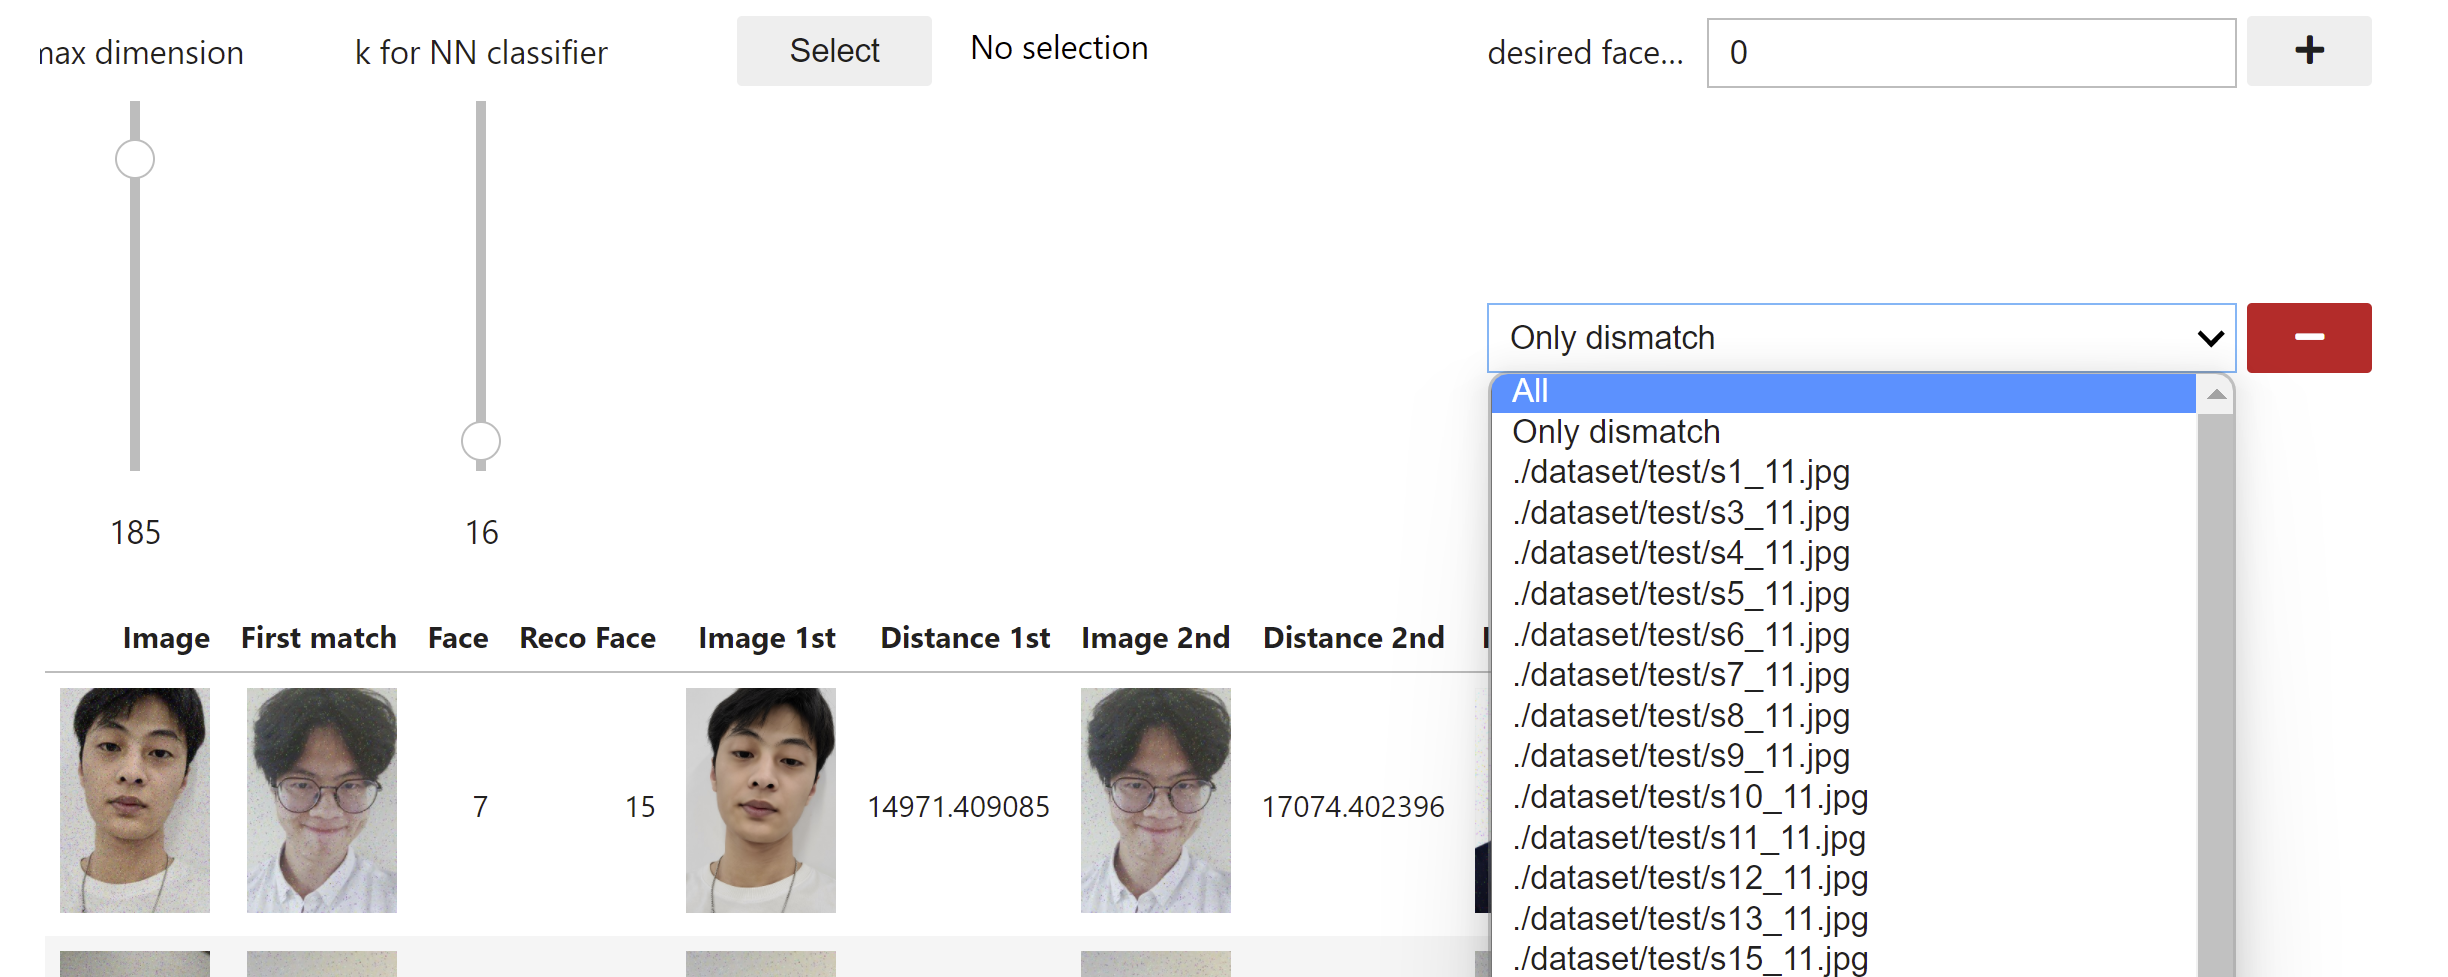
\includegraphics[width=.6\columnwidth]{ui2}
    \caption{第一个交互窗口展示特征向量重新投影至二维空间的情形,第二个交互窗口展示了分类的具体情况。}
    \label{fig:ui}
\end{figure}

第一个交互窗口允许用户选择一种matplotlib中定义了的颜色空间展示图像结果。根据\autoref{sec:eig}的结果,合适的颜色空间可让人眼更易于发现特定的数据区别。默认值无特定含义。

第二个交互窗口是一个动态加载的文件列表,默认加载所有测试集图片。在下拉框内可选择查看所有已加载文件,或是仅列出与样本标记不匹配的识别结果,抑或是选择单个文件。选择单个文件的环境下,用户可点击减号将该文件移出文件列表,也可以在上方选择文件后,给予相应的人脸标记,加入文件列表。配合对参数$k, d$的修改,本界面对系列识别结果有着直观的展示,同时非常适合用户调参和问题分析。

\section{开发工具选择}
\label{sec:dev}
本实验的基本要求是撰写Matlab源代码(\verb|.m|),并在算法实现的基础上完成一个可供用户使用的GUI界面。鉴于:1.在Python环境下numpy、pandas、scipy、matplotlib等宏包,对于Matlab在矩阵计算等方面的功能有较好的互补性和支持(\autoref{listing:dev});2.这些宏包配合ipython kernel与jupyter在开发及展示、移植上相较于Matlab更为方便;3.使用Python环境可以运用numba等工具,加速在中值滤波(\autoref{sec:median-filter0})等处使用到的循环流程,避免实现验证时的长时间等待,便于接轨实际应用。{\bfseries 因此,本实验的算法代码将以笔记本(\verb|.ipynb|)和Python源文件(\verb|.py|)的方式提供。}

同时,本节将对本次实验所用到的开发工具作简单的介绍,并重点分析其优势和它们之间的关系。使用方法此处不再赘述。

\begin{itemize}
\item 本实验代码的算法实现部分,大部分可经批量修改后由Matlab直接使用。例如以下两份节选代码,可实现对矩阵的相同操作。此处内置函数的实现方法(如\verb|eig|),在两种环境内也一般是使用LAPACK库。\cite{Tobler_2019, Numpy_eig}
\begin{listing}[!ht]
% https://www.overleaf.com/learn/latex/Code_Highlighting_with_minted
\begin{minted}[linenos, breaklines, tabsize=2, fontsize=\footnotesize]{matlab}
  [eigValue, eigPreVector] = eig(matMean .* matMean.T) % already sorted
  eigVector = (matMean.T .* eigPreVector) / eigValue
  eigNormalizedVector = eigVector / norm(eigVector, 0)
\end{minted}
\begin{minted}[linenos, breaklines, tabsize=2, fontsize=\footnotesize]{python}
  import numpy as np
  eigValue, eigPreVector = np.linalg.eig(np.dot(matMean, matMean.T)) # already sorted & normalized by eig function
  eigVector = np.dot(matMean.T, eigPreVector) / eigValue
  eigNormalizedVector = eigVector / npMat.norm(eigVector, axis = 0)
\end{minted}
\caption{对矩阵特征向量作转换后(\autoref{sec:pca0}),进行归一化处理(Matlab 和 Python 版本)}
\label{listing:dev}
\end{listing}

\item 使用\textbf{jupyter笔记本},可实现与Matlab相仿的代码、注释书写环境,并对生成数据进行实时终端处理,或是使用数据查看器进行进一步操作。
\begin{figure}[h]
    \centering
    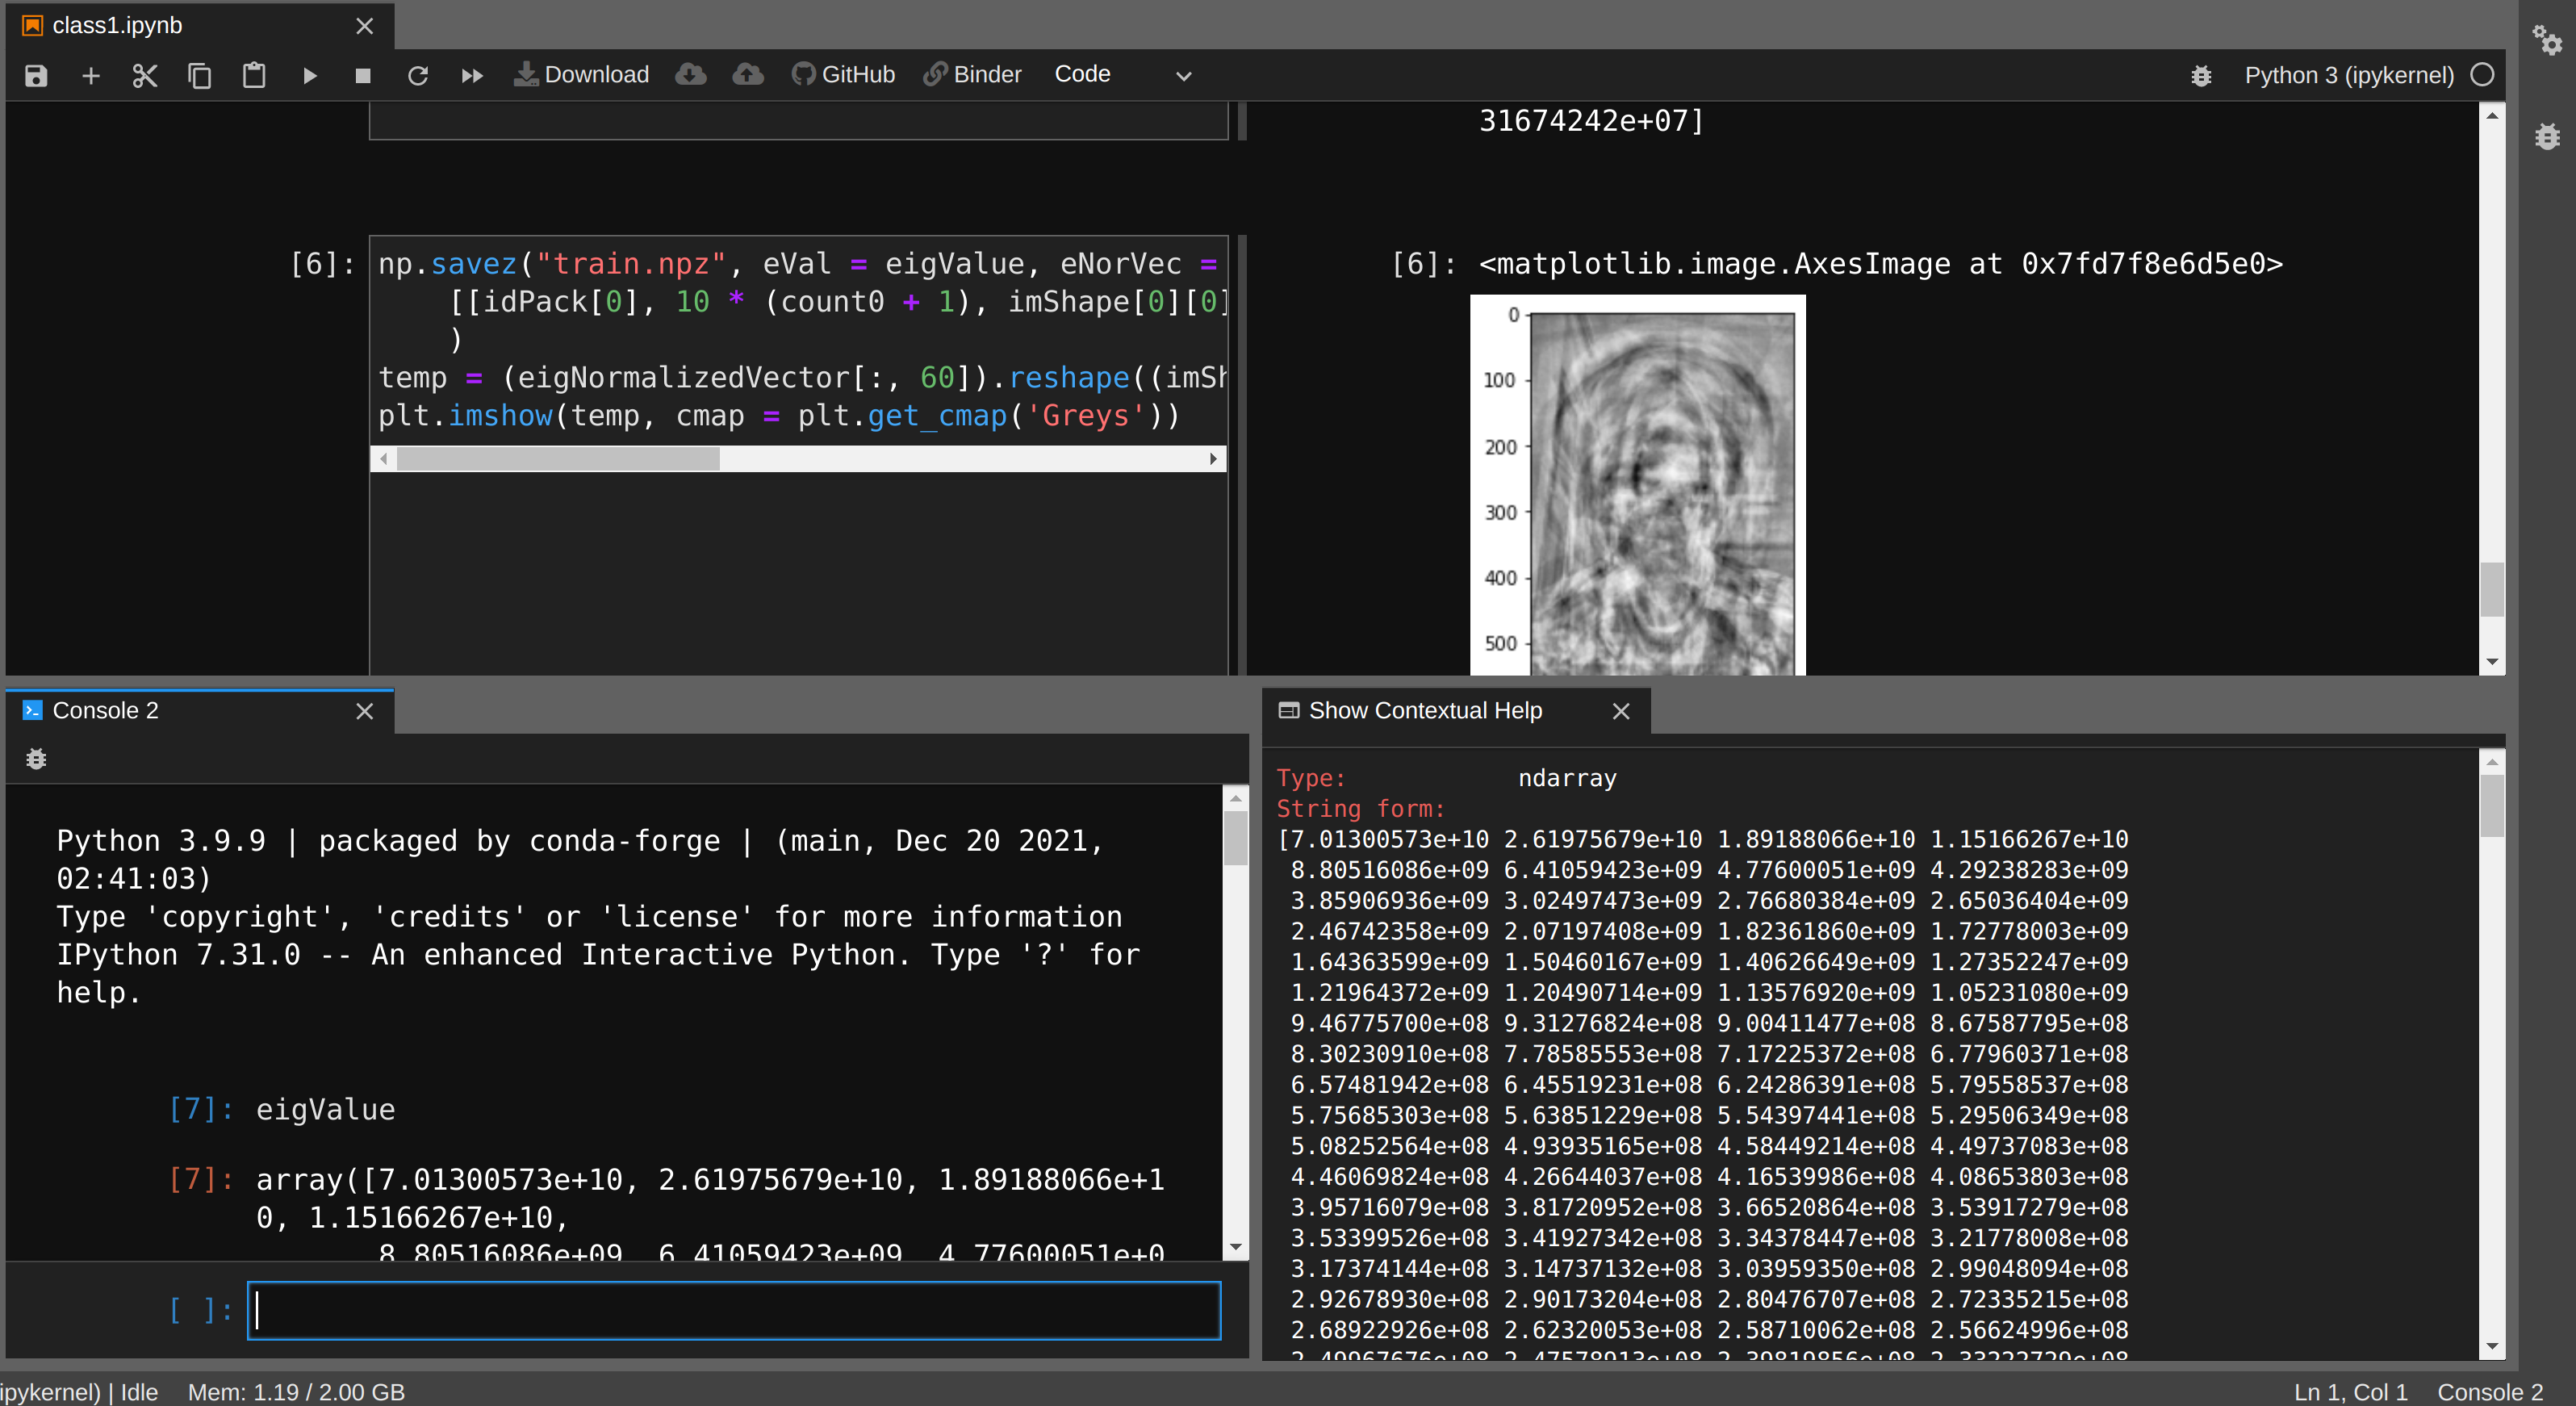
\includegraphics[width=0.9\columnwidth]{dev0.png}
    \caption{这是使用MyBinder平台,调用内核进行变量监测和查看帮助的界面。}
    \label{fig:jupyter-0}
\end{figure}
\begin{figure}[h]
    \centering
    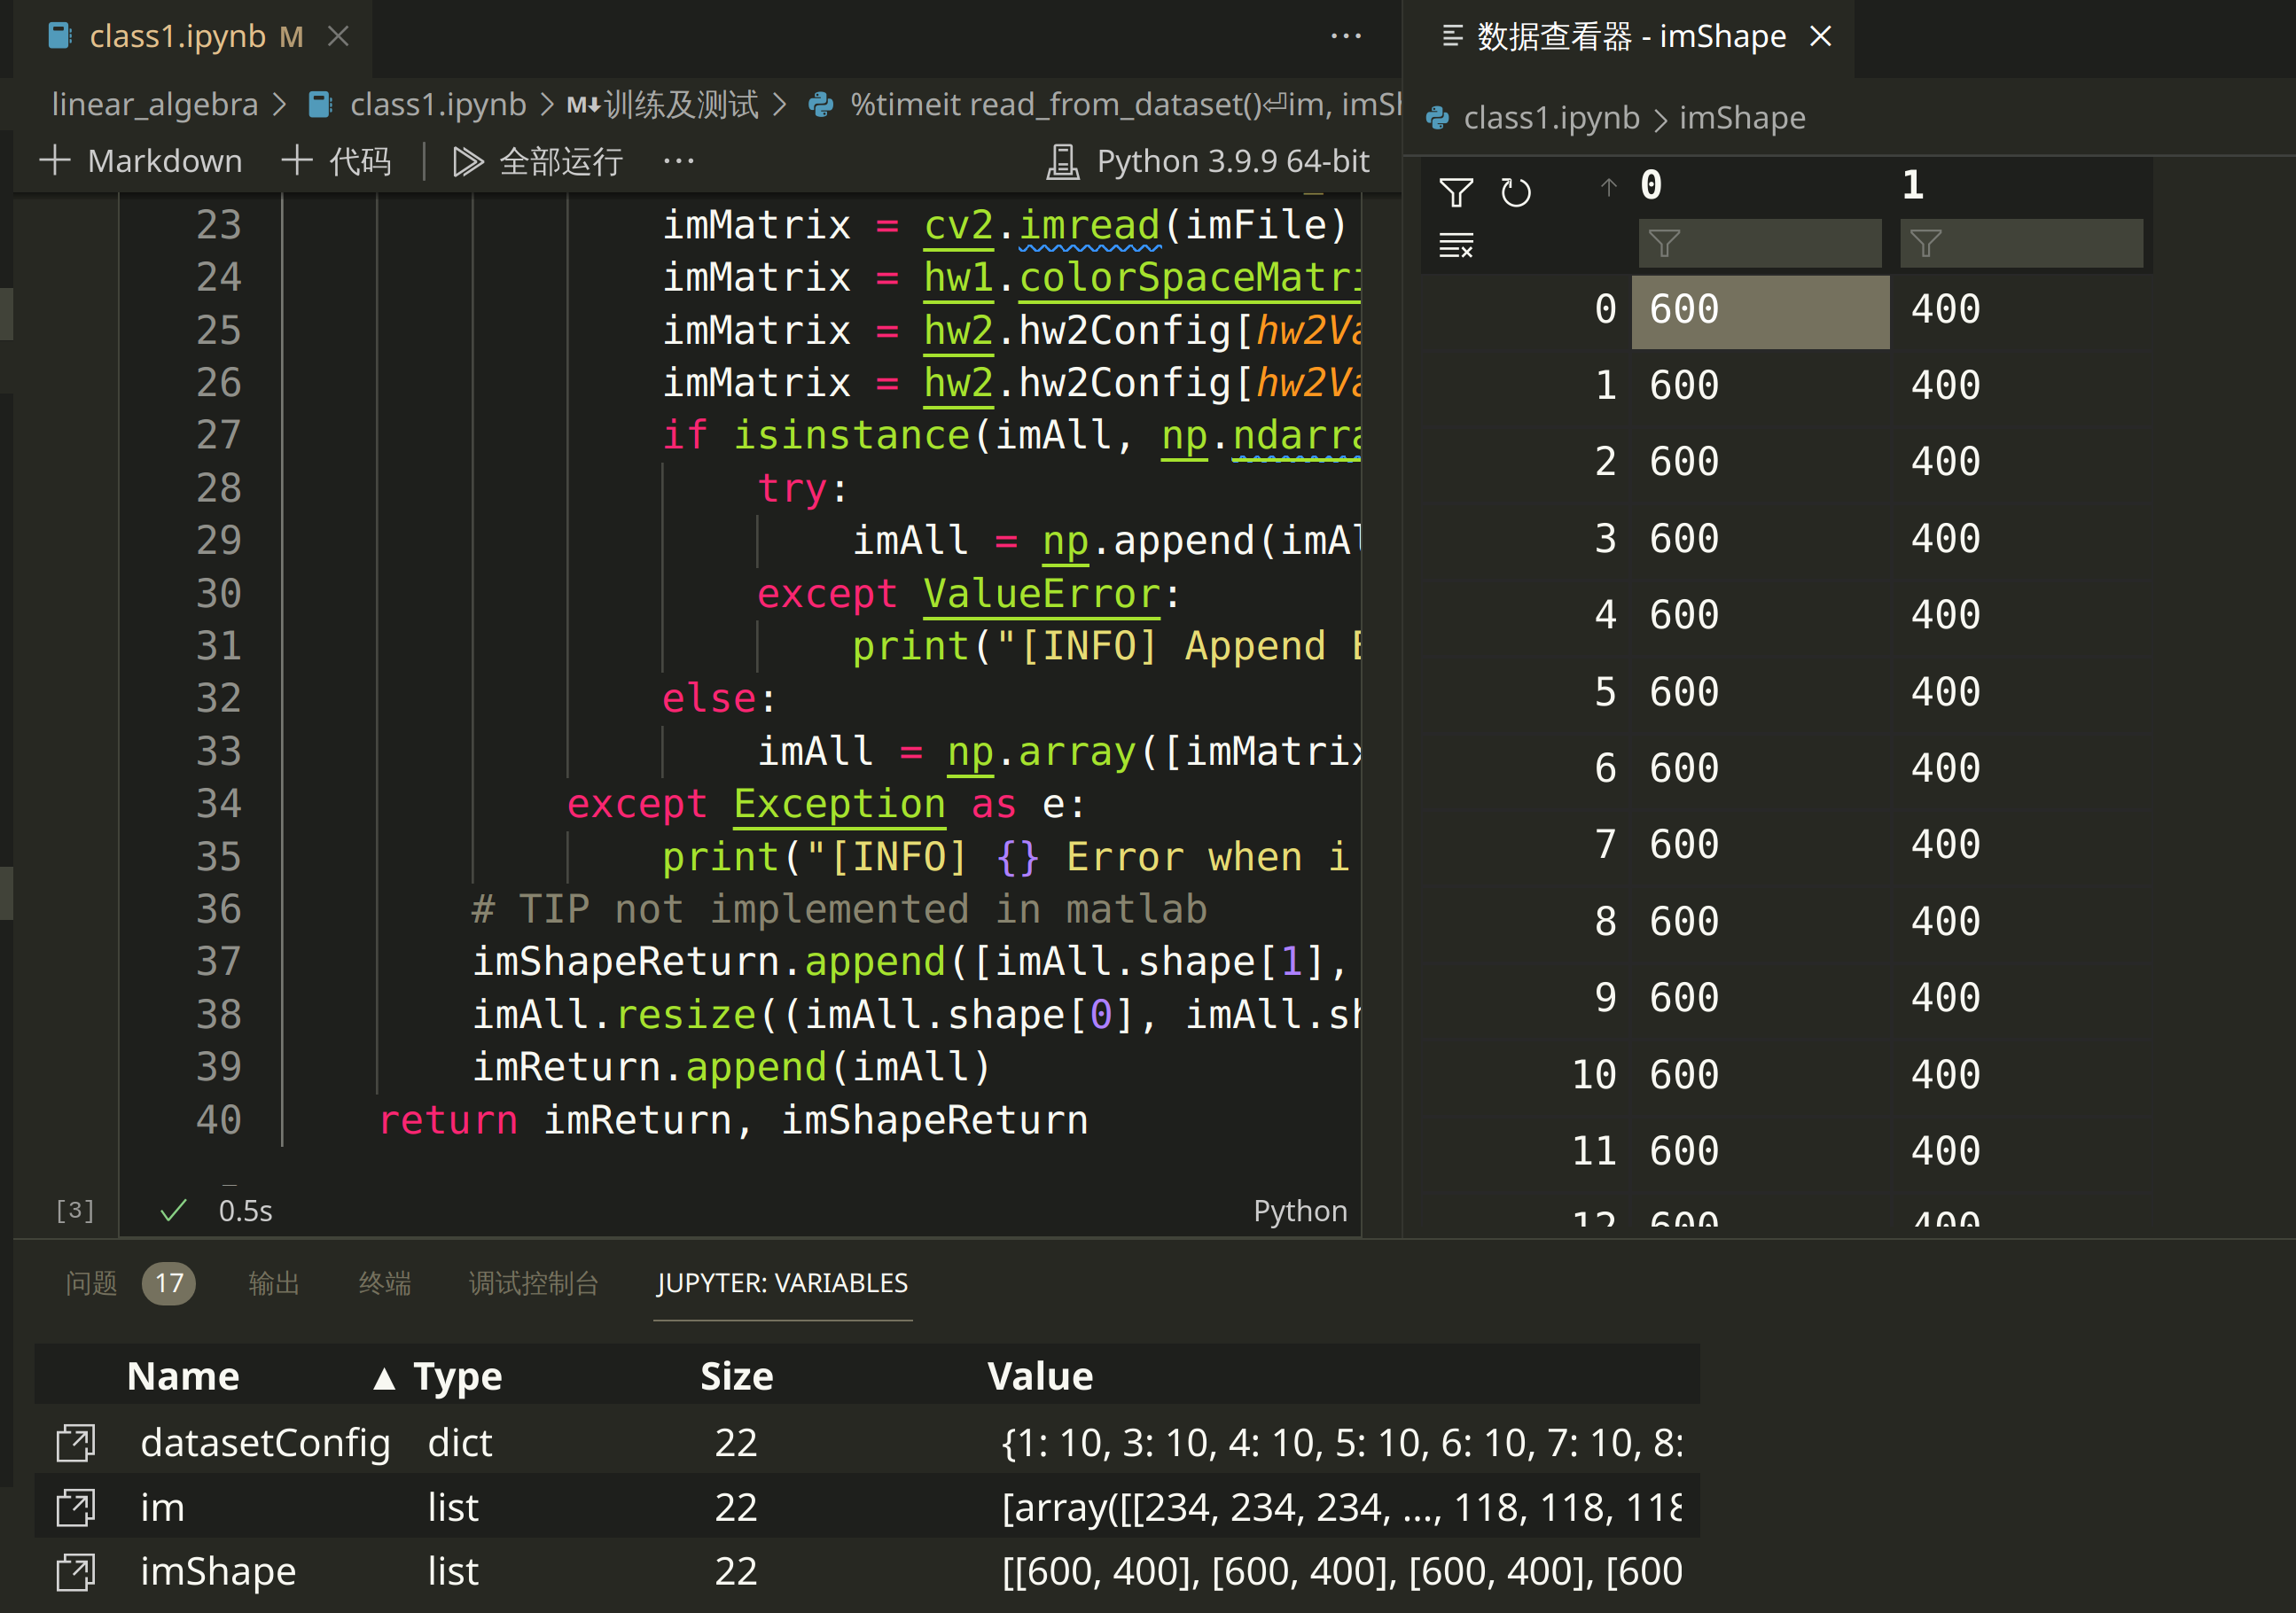
\includegraphics[width=0.9\columnwidth]{dev1.png}
    \caption{这是使用VS Code的Jupyter插件后\cite{Claudia_2021},概览数据(Data Viewer)的界面。}
    \label{fig:jupyter-1}
\end{figure}

\item \textbf{numpy}宏包是Python环境下进行矩阵运算的主流工具,与之相对应的是用于深度学习计算的\textsf{pytorch}宏包,该宏包与numpy的矩阵/张量相兼容。使用numpy宏包时,要尽可能使用自建函数代替循环,以避免动态语言执行耗时。\cite{Numpy_multi_dot}

\textbf{scipy}宏包对高阶方程运算等提供了支持。numpy.linalg依赖本包。

\textbf{scikit-learn}宏包适用于初学者对机器学习的各类工具进行直接调用。

\item \textbf{pandas}宏包完善了二维数据的可视化相关功能。\cite{GeeksForGeeks_2020}

\textbf{matplotlib}宏包完善了各类型的基本作图方法。

\textbf{opencv}宏包提供图片显示,以及跨系统的简易UI窗口创建及布局支持。

\item \textbf{实验代码预留了网络交互接口,可开发对应的GUI界面。}为了提供跨平台的支持,程序只提供静态的网站内容和数据流接口,便可达成使用手机摄像头等多设备,测试该程序的目的。这是利用Matlab难以完成的。

\item \textbf{numba}宏包基于numpy,可以通过预编译加速\verb|for loop|等费时的操作。
\end{itemize}
\chapter{实验结果及分析、讨论}
\label{cha:re}

本章展示的实验数据,可通过调用程序相应部分复现。实验分析部分基于文献搜索结果。

\section{模块单元结果}

\subsection{图像的滤波处理}

对某相机拍摄的PNG图片,读取RGB颜色空间后,处理效果如\autoref{fig:hw1}:(其中从左上角,以先从左到右,再从上到下的顺序标数,第一张图像为原图,第二张图像为最大值取样,第三张图像为平均值取样,第四张图像为加权平均值取样(Luminance))

\begin{figure}[H]
    \centering
    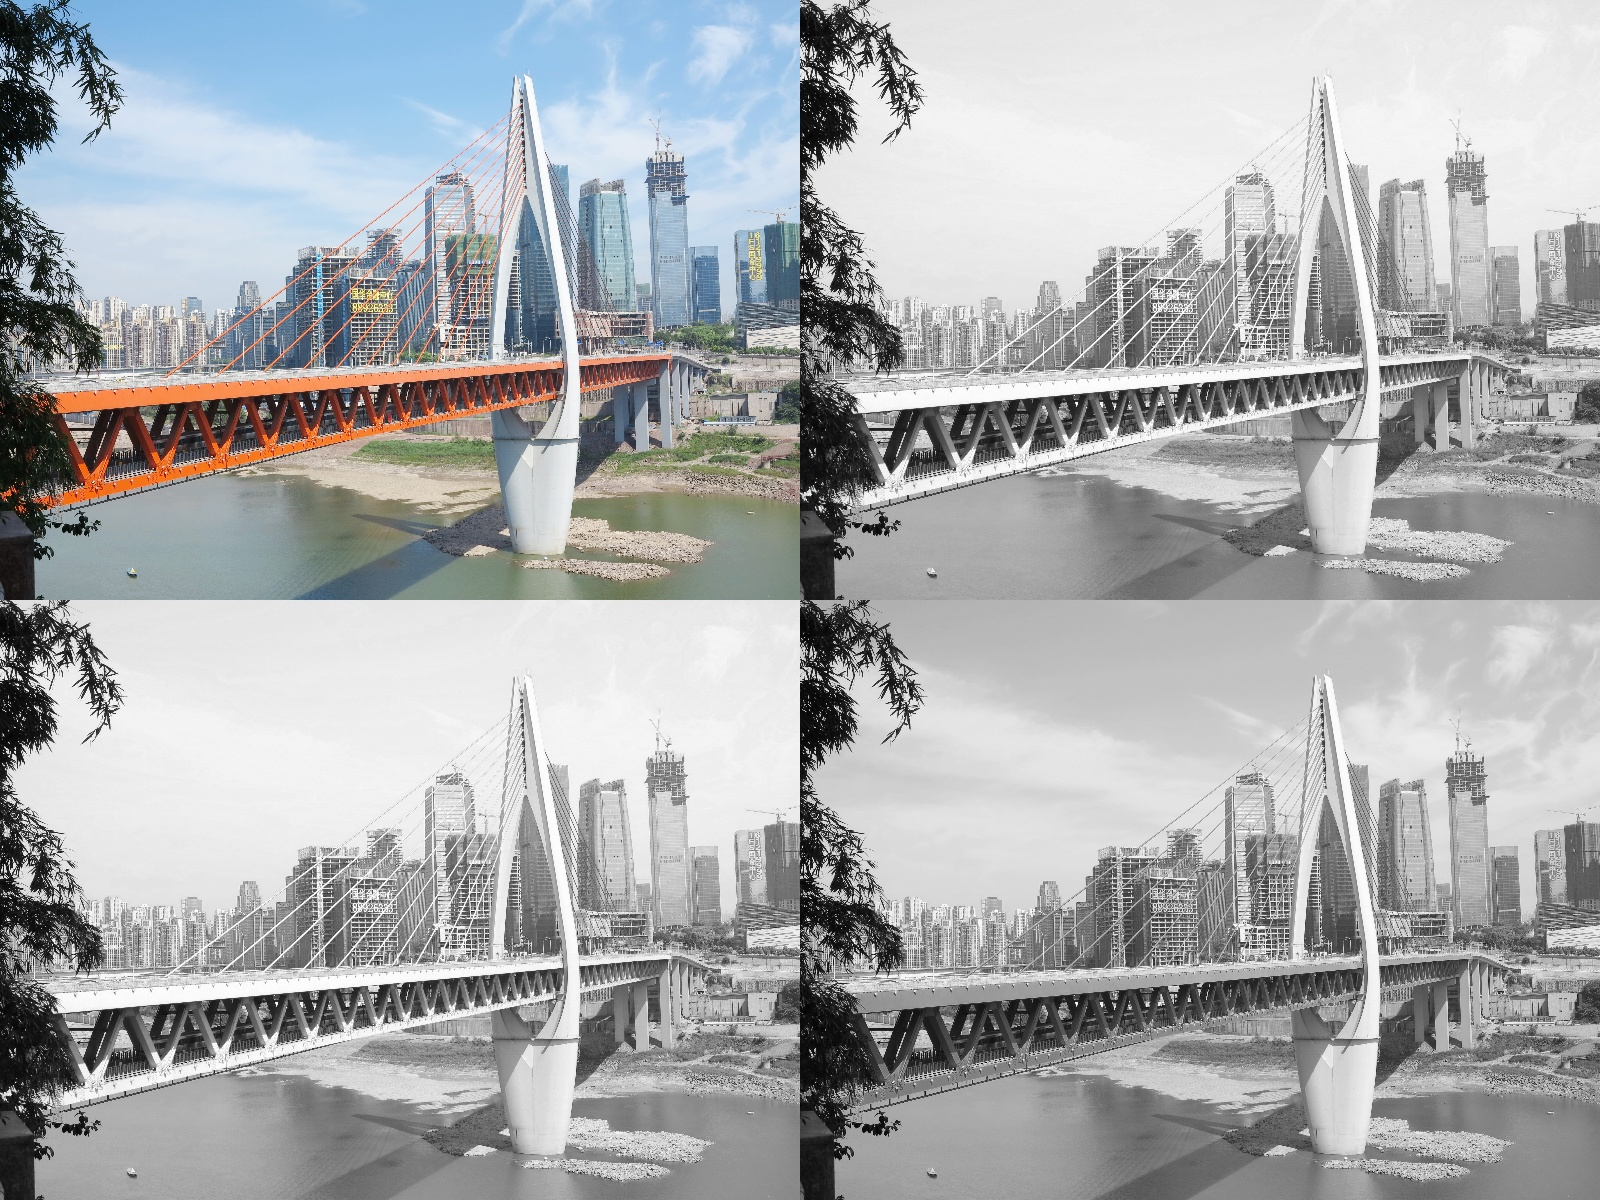
\includegraphics[width=.5\columnwidth]{hw1.jpg}
    \caption{灰度处理实验结果}
    \label{fig:hw1}
\end{figure}

根据人眼观察,在这种情况进行灰度空间转换时,使用加权平均值取样对这张图片的还原度最大,其明度较高的细节,如蓝天白云、红色桥梁等得到了充分保留。而后对数据库内人脸进行同等处理,也得到类似的直观结论。(所以电子行业用这个标准,还是有原因的!)

另外,在使用MATLAB或Python numpy库直接对读取图像进行处理时,很容易忽略数据类型的问题。对于正常的8位3通道图片,各像素点的数据均以\verb|uint8|的形式储存,在加权求和时,由于人脸数据库中图片明度普遍较高,故通道先求和,所得值将超过$2^8-1=255$,导致结果图像数据失真。可以调用平均值函数,或者数据类型转换来无损的解决这个问题。

需要注意的是,若要对这一结果进行深入研究,除了分析观察值外,还要结合其应用场景进行分析。此处,鉴于主流的图像处理工具(Matlab, OpenCV)均使用了Luminance加权平均值取样,故不再具体探讨其对实验结果的影响。为直击重点,本实验也不再探讨直方图优化、伽玛校正的原理,及其与灰度转换相结合的具体作用效果。

\begin{figure}[H]
    \centering
    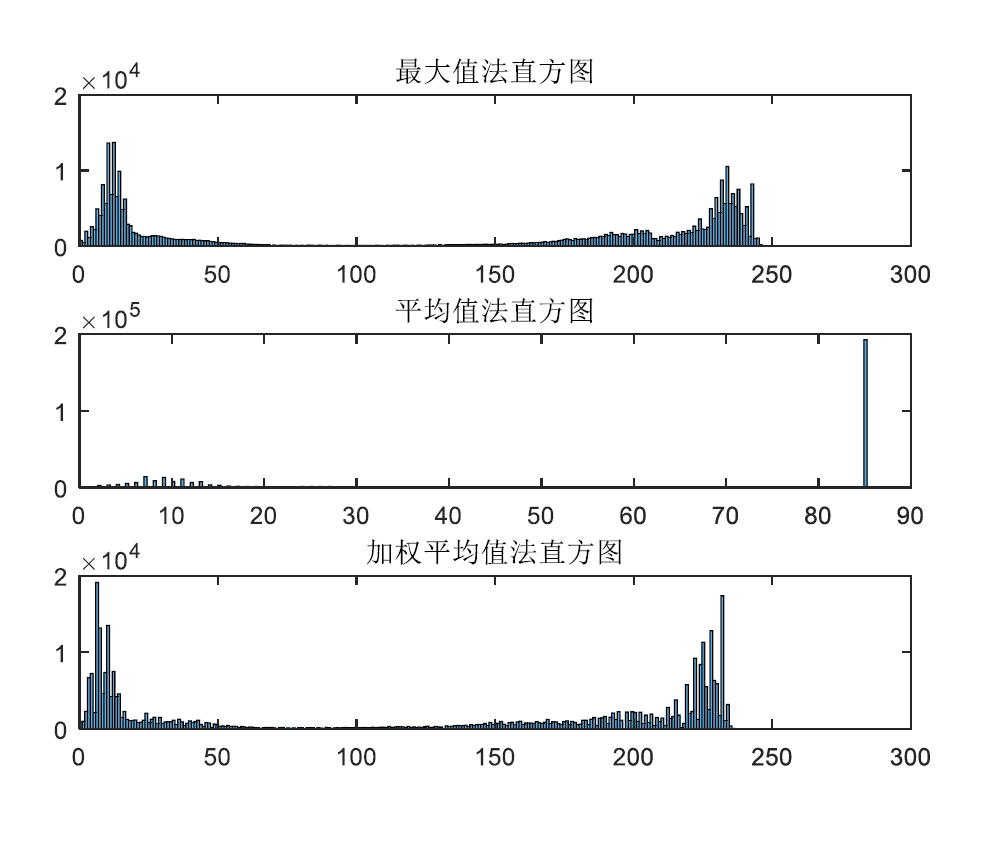
\includegraphics[width=.5\columnwidth]{hw1_add.png}
    \caption{某人脸图片经不同灰度处理后的直方图结果}
    \label{fig:hw1_add}
\end{figure}

\textbf{综上,经分析,程序主模块最终采用本部分的加权平均值取样部分(浮点输出)。}

\subsection{图像的主成分分析}

对数据库中训练库、测试库中的部分照片进行多种去噪处理,并将其图片输出,过中心的平行、垂直线上像素的R通道值的绘图数据,各像素点R通道8位值数据的直方图制作成图表,结果如下。

\begin{figure}[H]
    \centering
    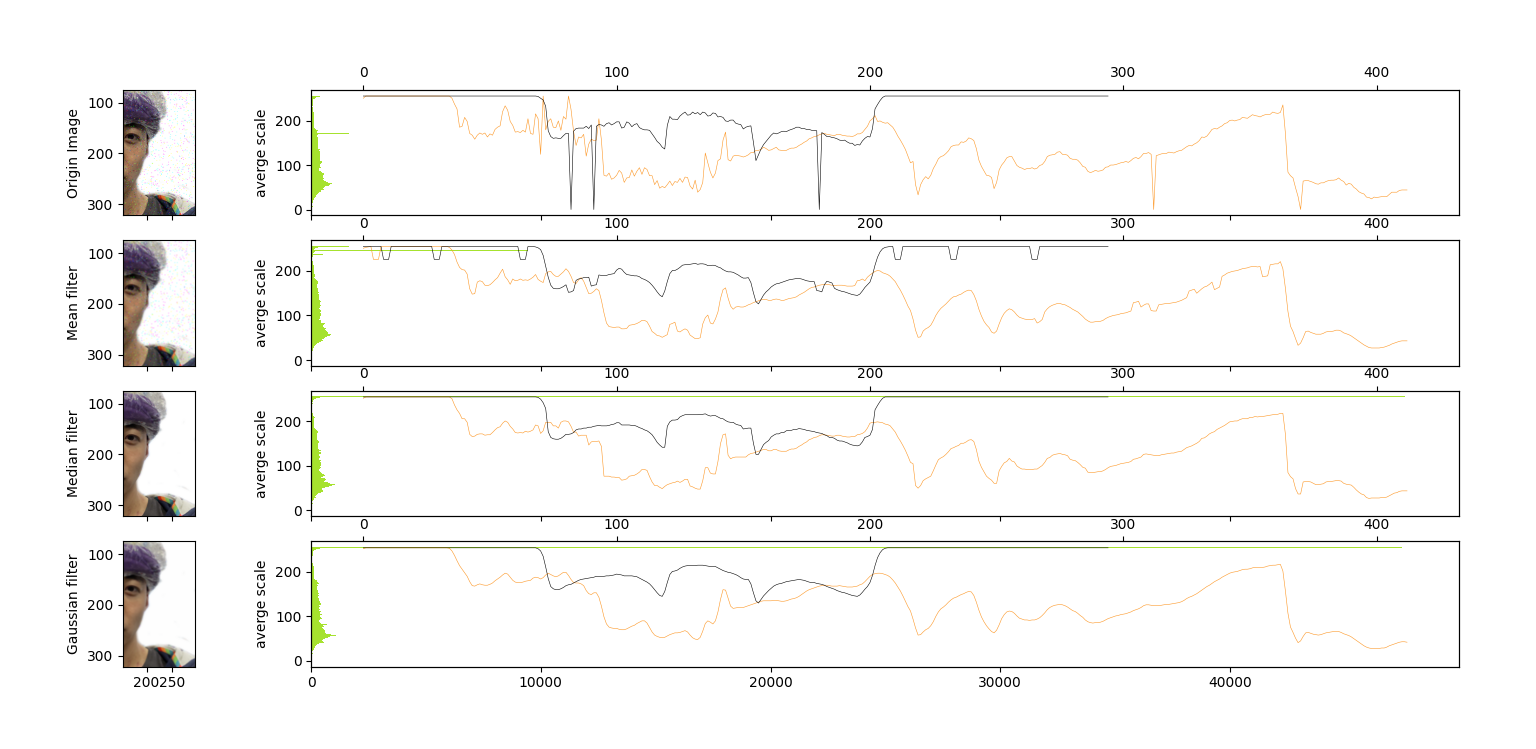
\includegraphics[width=.81\columnwidth]{hw2_fig1.png}
    \caption{三种滤波处理后的输出结果}
    \label{fig:hw2_1}
\end{figure}

\begin{figure}[H]
    \centering
    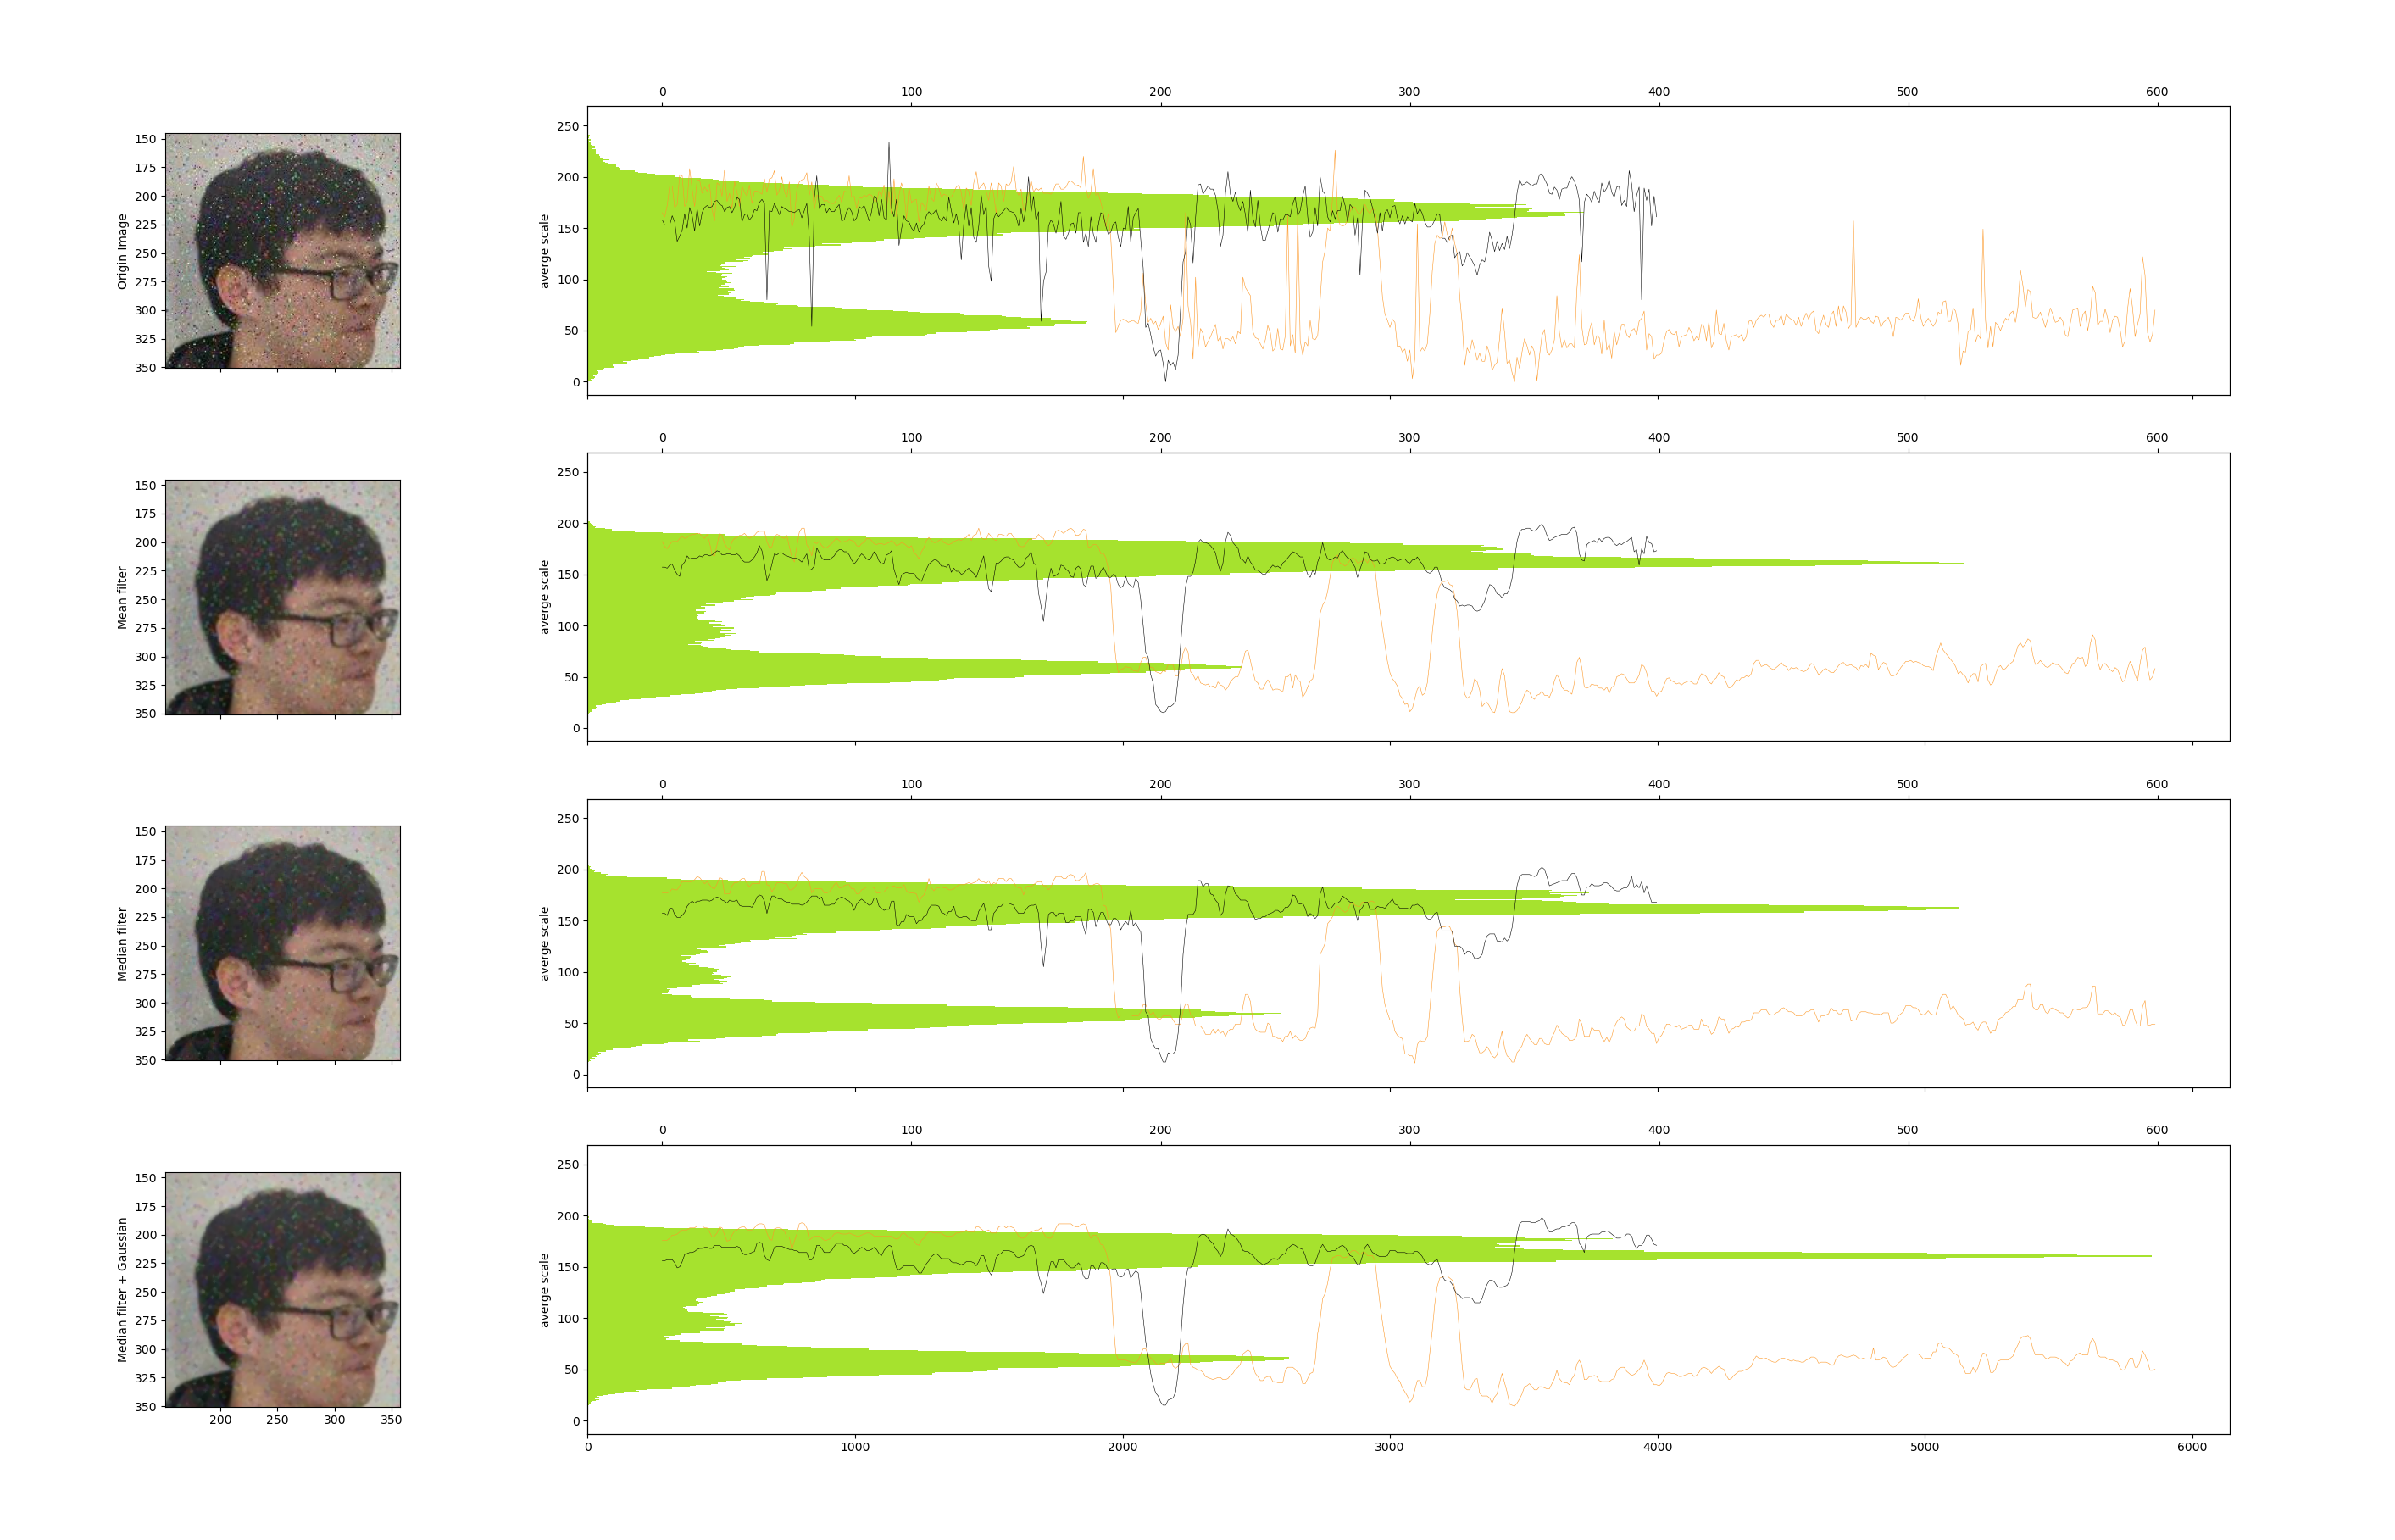
\includegraphics[width=.81\columnwidth]{hw2_fig2.png}
    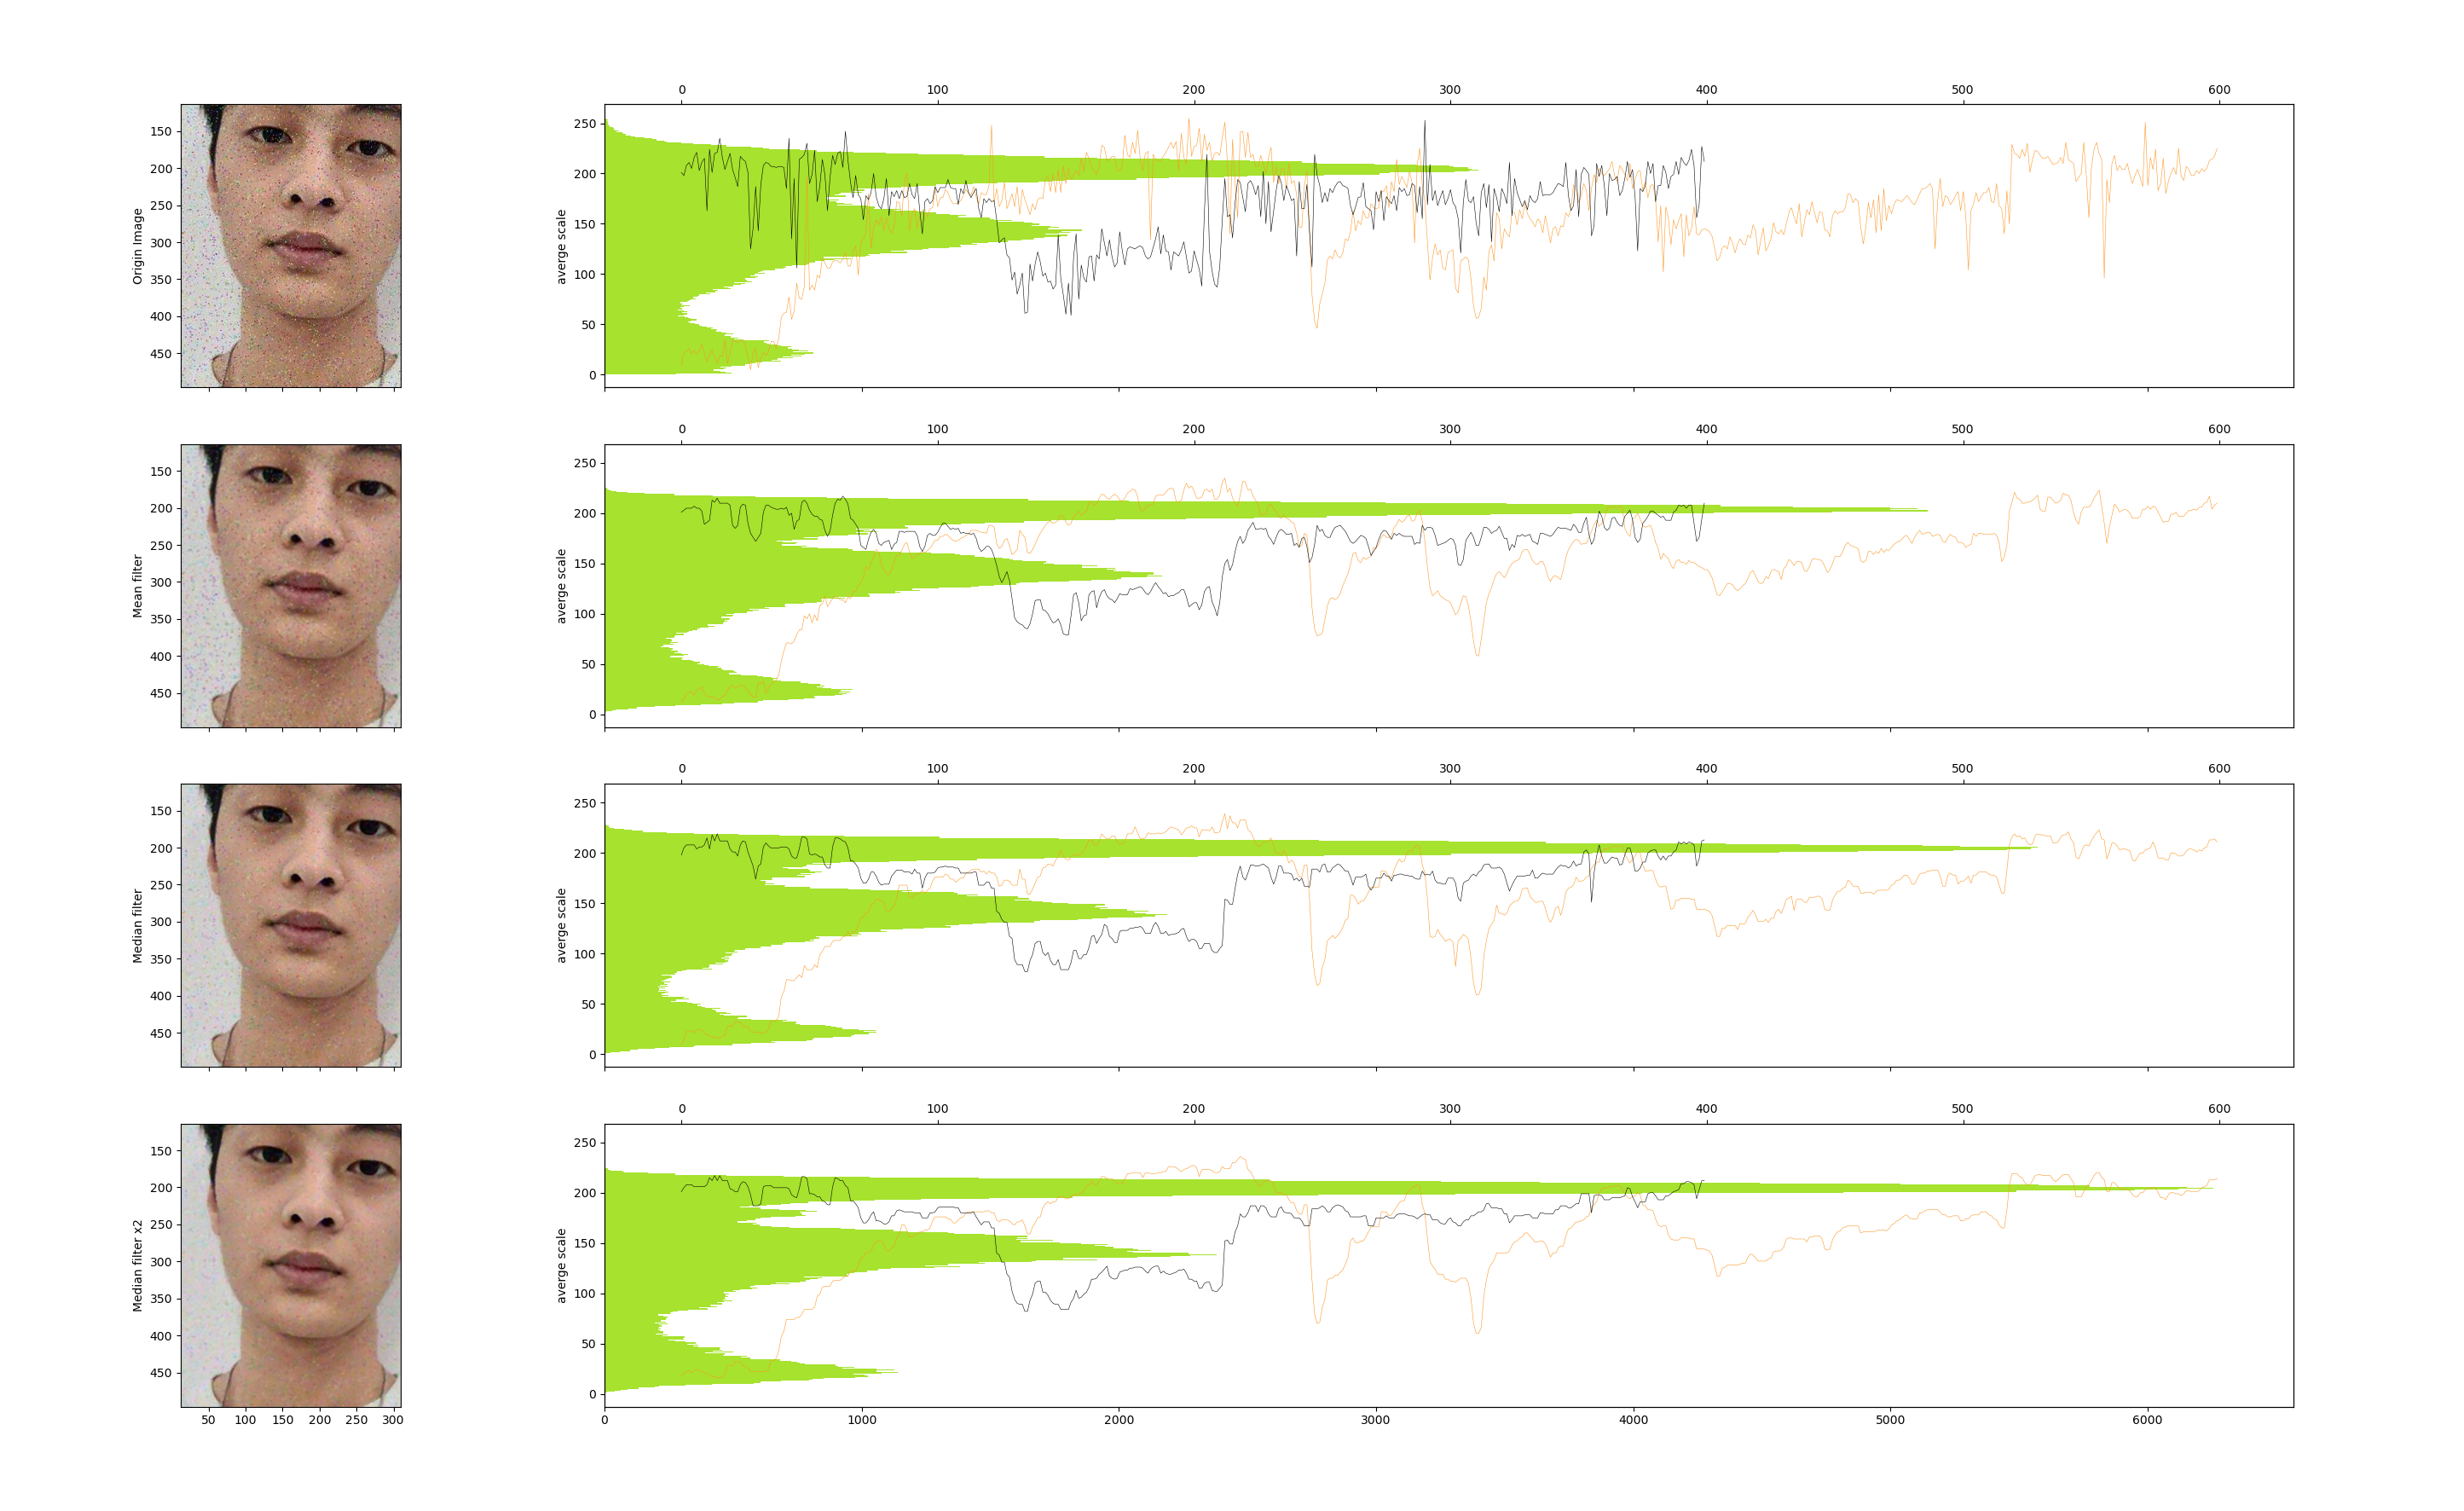
\includegraphics[width=.81\columnwidth]{hw2_fig3.png}
    \caption{分别展示了高斯滤波后中值滤波,两次中值滤波的输出结果}
    \label{fig:hw2_2}
\end{figure}

\autoref{fig:hw2_1}自上而下,展示了原图、均值滤波、中值滤波、高斯滤波的相应结果。可以发现均值滤波对椒盐噪声去除效果不好,另外两种滤波对简单的椒盐噪声去除效果较好。

\autoref{fig:hw2_2}的第一张后两行展示的分别是中值滤波、高斯滤波后中值滤波的输出结果,可以发现高斯滤波反而会增强高密度的椒盐噪声。其第二张后两行展示的分别是一次中值滤波、两次中值滤波的输出结果,可以发现二次中值滤波对噪声还有一定的削减作用。次数再次升高后,效果不再明显。

\textbf{综上,经分析,程序主模块最终采用本部分的中值滤波,并连续调用两次。}

\section{识别、交互系统结果}

\subsection{处理时间}
\label{sec:pca0}

\textbf{在本机}统计了训练模块中较为耗时的两部分:中值滤波处理和样本库主成分分析。不采用中值滤波的耗时为3.4\~4.9s,采用未加速的中值滤波耗时约为18min51s(每张图耗时约5s),numba加速的中值滤波耗时为15.5\~20.4s;主成分分析的耗时为4.2\~9.1s。

识别模块中耗时的主要部分为测试集批量读入,可同等看待。

\begin{figure}[h]
    \centering
    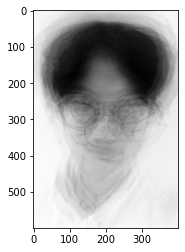
\includegraphics[width=.4\columnwidth]{eig_single.png}
    \caption{单组样本训练得到的第一个主特征,经可视化处理。}
    \label{fig:eig_single}
\end{figure}

\subsection{识别准确度}

对kNN分类算法和选取的主成分进行调整,发现当 $k=4$ 时,主成分最少仅需容纳前$12$维即可达到最佳识别正确率。仅\autoref{fig:class1}所示的样本无法被正确识别。增大主成分维数,识别结果基本不受影响。而增大 $k$ 值会导致部分测试样本匹配到其他类型的人脸。

样本12在$k$、$d$较高时才能被正常识别,如$k=27, d=185$。故样本12的训练集有过拟合的倾向。

\begin{figure}[H]
    \centering
    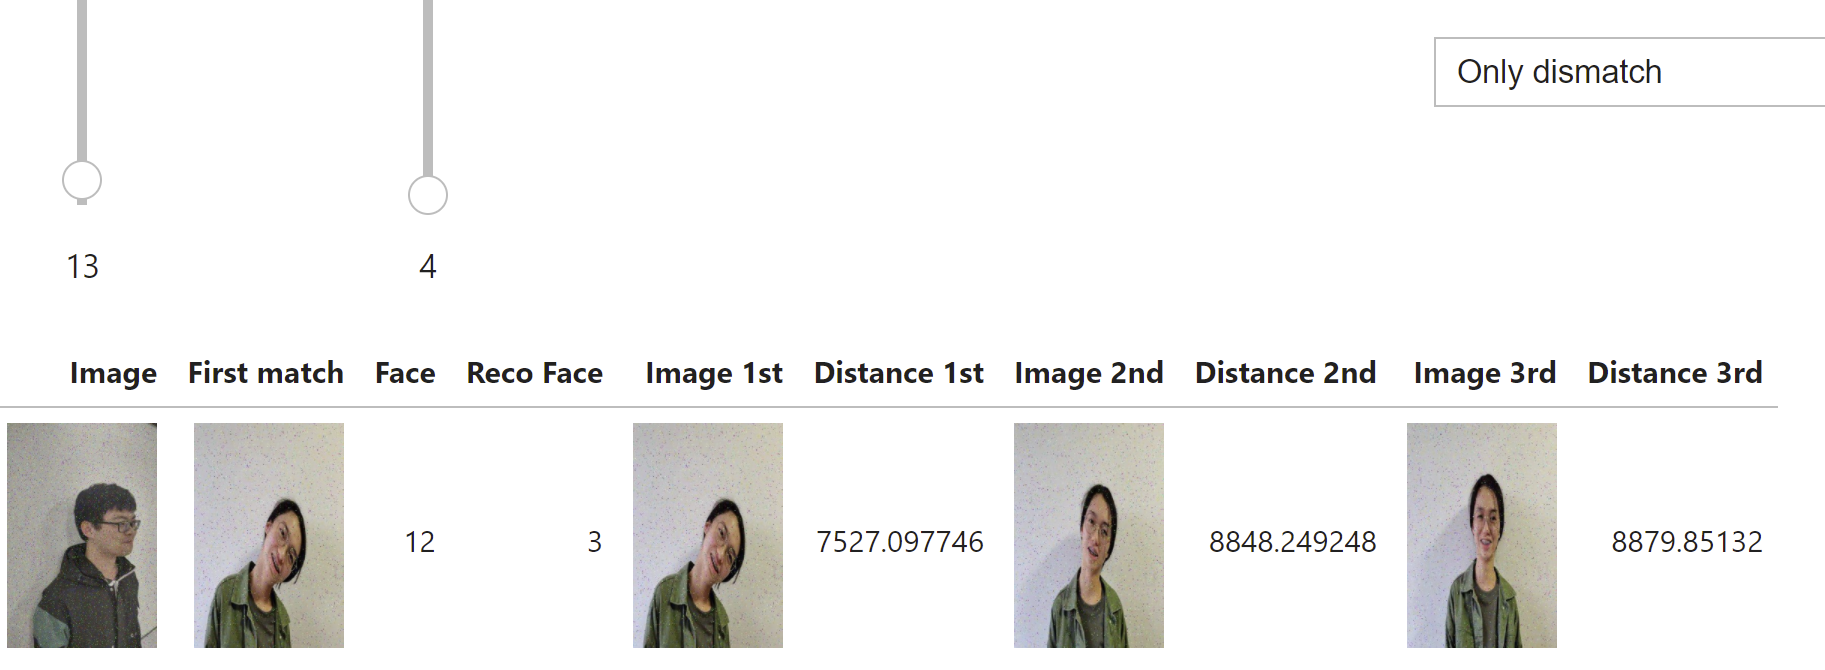
\includegraphics[width=.8\columnwidth]{class1.png}
    \caption{无法匹配的样本图片和识别输出结果}
    \label{fig:class1}
\end{figure}

\section{识别的调整及优化}

下列的数据展示了选取前$d$维主成分和$k$个临近数据集点后的分类情况。注意到有部分测试数据十分接近于训练数据,经查看文件,其中有部分测试图片与训练图片完全一样,另有一些是噪声不同。

\begin{minted}[breaklines]{xml}
d=20, k=4
test face 3 is too close to dataset(s3_1)?
test face 4 is too close to dataset(s4_3)?
test face 9 is too close to dataset(s9_1)?
12 3 [[9.92052951e+03 1.60000000e+01 3.00000000e+00]
 [9.92129420e+03 1.90000000e+01 3.00000000e+00]
 [1.06769758e+04 1.88000000e+02 2.40000000e+01]
 [1.06920015e+04 1.80000000e+01 3.00000000e+00]]
test face 22 is too close to dataset(s22_3)?
Error rate is 0.05.

d=120, k=4
test face 3 is too close to dataset(s3_1)?
7 15 [[[1.41684977e+04 5.80000000e+01 7.00000000e+00]
 [1.62357532e+04 1.23000000e+02 1.50000000e+01]
 [1.70395660e+04 1.20000000e+02 1.30000000e+01]
 [1.92705277e+04 1.22000000e+02 1.50000000e+01]]
test face 9 is too close to dataset(s9_1)?
12 3 [[1.61600607e+04 1.80000000e+01 3.00000000e+00]
 [1.71320333e+04 1.88000000e+02 2.40000000e+01]
 [1.71812421e+04 1.00000000e+01 1.00000000e+00]
 [1.78519738e+04 1.60000000e+01 3.00000000e+00]]
 test face 22 is too close to dataset(s22_3)?
Error rate is 0.1.
\end{minted}

那么我们拿完全不滤去噪声的训练集和测试集来跑跑看呢?好家伙,噪声似乎真的被当作一个特征,留存在高维度的主成分里了。只考虑低维度的主成分,噪声对分类的影响反而不大。

\begin{minted}[breaklines]{xml}
d=6, k=5
test face 1 is too close to dataset(s1_7)?
test face 3 is too close to dataset(s3_1)?
test face 9 is too close to dataset(s9_1)?
13 12 [[ 6279.65703444   175.            23.        ] [11301.58253784   102.            12.        ]]
test face 22 is too close to dataset(s22_3)?
23 5 [[ 8416.09473533   171.            23.        ] [10590.35552612   174.            23.        ]]
Error rate is 0.1.

d=100, k=5
6 3 [[1.34565528e+04 4.40000000e+01 6.00000000e+00] [1.50439833e+04 4.50000000e+01 6.00000000e+00]]
7 15 [[9.86112416e+03 5.80000000e+01 7.00000000e+00] [1.64500187e+04 1.22000000e+02 1.50000000e+01]]
8 22 [[10763.33564653   163.            22.        ] [12367.46637443   162.            22.        ]]
test face 9 is too close to dataset(s9_1)?
13 23 [[2.06595640e+04 1.75000000e+02 2.30000000e+01] [2.58334201e+04 1.70000000e+02 2.20000000e+01]]
23 5 [[2.16220804e+04 1.71000000e+02 2.30000000e+01] [2.55125896e+04 3.20000000e+01 5.00000000e+00]]
Error rate is 0.25.
\end{minted}

\subsection{生成特征向量分析}
\label{sec:eig}

将中值滤波前后的主成分分析工具:特征向量进行比较,更可以发现一些有趣的现象。

\begin{figure}[H]
    \centering
    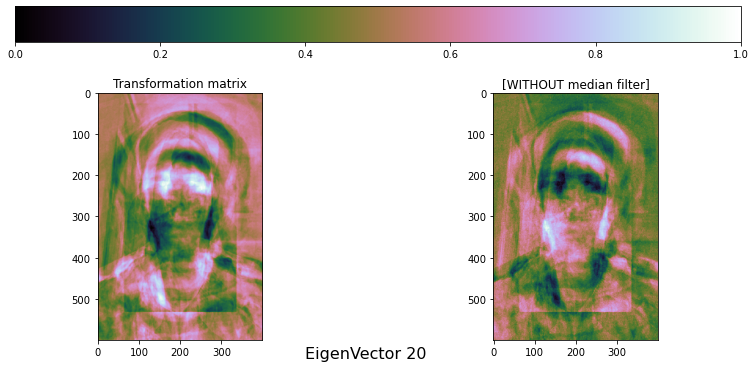
\includegraphics[width=.8\columnwidth]{eig_20.png}
    \caption{$d=20$时的特征向量输出}
    \label{fig:eig_20}
\end{figure}

颜色空间是按照百分比的方式(0~1)对归一化的特征向量进行绘制的。不同方式生成的特征向量,有时候会接近相似,有时会大相径庭,但有时候却会……完全相反?

\begin{figure}[H]
    \centering
    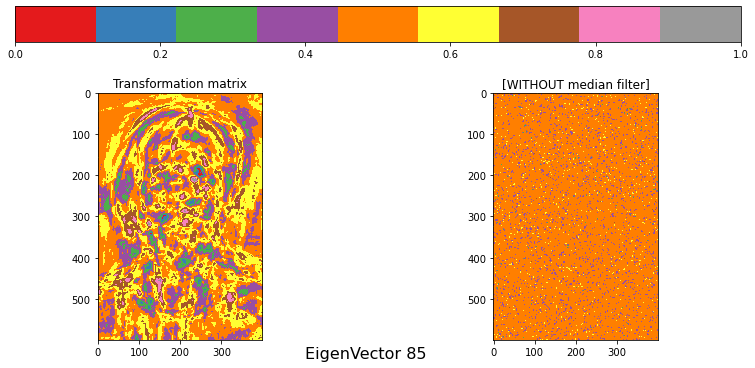
\includegraphics[width=.8\columnwidth]{eig1.png}
    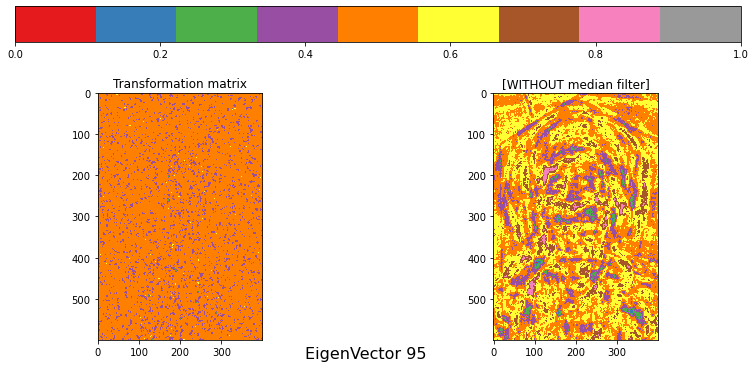
\includegraphics[width=.8\columnwidth]{eig2.png}
    \caption{$d=85$和$d=95$时的特征向量输出}
    \label{fig:eig}
\end{figure}

随着维数增大,两种特征向量里都出现了噪声形成的主成分,且中值滤波前的主成分为噪声的维数更多。这说明生成的噪声过于密集,造成了两个结果:

1.噪声重合形成了一定的规律,并被代数方法所单独识别出来。(这听上去就很无监督学习。)否则,噪声应基本在含有人脸的特征向量中显现。(实际上,两种特征向量里也都有这种情况)

2.套用的中值滤波方式仍不能很好的去除现有的噪声。

那么是时候总结一下了。
\chapter{反思与总结}

总结本阶段实验,第一项实验给我留下了最深刻的印象。在我之前的认识中,图像的预处理在不同应用领域应当都有最常用的实现方式,甚至于可证明的最优解(State of art)。然后发现这里面的水还是太深了……要考虑的内容比神经网络相关的具体太多,而不是虚无缥缈地调参。同时,我甚至一直以为色彩转灰度只是简单的平均数计算,但对比的图像及其相应的结果都让人大吃一惊。这说明了人眼很容易被图像诓骗,但它又经常对变化敏感。那么,文献收下了,咱慢慢看。

在整理实验报告的时候才注意到滤波器还有很重要的一点没有考虑到,即其作用范围(滤波子的大小)。中值滤波选用稍大的滤波子时,可能会对该数据集的噪声有显著提升的抑制作用。但噪声最好也得用个工具,从信号的角度出发,量化测量一下,不然又得用肉眼看?这可不太好。

在本实验中,数据集有过拟合倾向,因此还应考虑选用其他人脸数据集进行测试,这样或许也能进一步验证我的猜想。不过本次实验也让我迷迷糊糊地认识了协方差矩阵这一个重要概念,老朋友以后见!

感谢老师、助教、同学和开源资料,以及所引参考文献的各作者。该实验的完成缺少不了你们的贡献。

\backmatter %%% 后置部分(致谢、参考文献、附录等)


%% 致谢
% \include{contents/ack}
%% 参考文献
% 顺序编码制:cqunumerical		
% 注意:至少需要引用一篇参考文献,否则下面两行会引起编译错误。
\bibliographystyle{cqunumerical}
\bibliography{pca}

\chapter{附\hskip\ccwd{}录}
\section{程序源代码}

\begin{figure}[htb]
	\dirtree{%
		.1 \myfolder{pink}{工作文件夹}.
		.2 \myfolder{cyan}{class1.ipynb}.
		.2 \myfolder{cyan}{recognition.ipynb}.
		.2 \myfolder{cyan}{hw1.py}.
		.2 \myfolder{cyan}{hw2.py}.
		.2 \myfolder{cyan}{dataset}.
		.3 \myfolder{lime}{s1}.
		.3 \myfolder{lime}{...}.
		.3 \myfolder{lime}{test}.
	}%\dirtree
\caption[]{软件源代码文件结构图示。}
\label{fig:filetree}
\end{figure}

另可见\url{https://github.com/Tiger3018/hw/tree/HEAD/linear_algebra}。

\verb|hw1.py|: 图像的灰度处理
\inputminted{python}{./code/hw1.py}
\verb|hw2.py|: 图像的滤波处理
\inputminted{python}{./code/hw2.py}
\verb|class1.ipynb|: 图像的主成分分析,训练模块。
\inputminted{python}{./code/class1.ipynb}
\verb|recognition.ipynb|: 分类模块:可视化的训练数据读取及识别分类
\inputminted{python}{./code/recognition.ipynb}

\section{在线运行}

可以访问\url{https://mybinder.org/v2/gh/tiger3018/hw/89041d1?labpath=linear_algebra\%2class1.ipynb},快速实现视频中展示的所有软件功能。只需注意:

\begin{itemize}
    \item 需要一个稳定的网络环境。
    \item 分配得到的虚拟环境内存需要为2GB。当分配到的内存仅有1GB时,不能正常生成训练结果。
    \item 请将训练模块中的计时部分(\verb|%timeit|)注释(\verb|#|)。出现的计时部分在云端运行一次,分别需要约30秒和20秒。
\end{itemize}

要生成训练结果\verb|train.npz|,请完全运行一次\verb|class1.ipynb|。在生成训练结果或上传训练结果后,再完全运行一次\verb|recognition.ipynb|,即可展示可交互界面。

%\begin{table}[htb]

%\begin{equation}
%\alpha\beta\gamma\delta\epsilon\varepsilon\zeta\eta = CD\Gamma\varGamma Z
%\end{equation}\eqlist{附录中的公式编号2,双语}[Equation name in English B]

%测试用途:theequation值为:\theequation ,thefigure值为:\thefigure ,thetable值为:\thetable


\end{document}